\pdfminorversion=7
\documentclass[
    11pt,
    a4paper,
    sfdefaults=false,
    toc=chapterentrywithdots,
    twoside,openright,
    titlepage,
    parskip=half,
    headings=normal,  % reduces heading size
    listof=totoc,
    bibliography=totoc,
    index=totoc,
    captions=tableheading,  % caption below table
    chapterprefix,
    listof=flat,
    final
]{scrbook}


% details about your thesis
\newcommand{\titel}{KI-gestützte Transformation statischer in interaktive 3D-Objekte durch Benutzerinteraktion}
\newcommand{\artderarbeit}{Bachelorarbeit}  % {Bachelorarbeit,Masterarbeit}
\newcommand{\autor}{Friedrich Allenhof}
\newcommand{\studiengang}{Medieninformatik}  % {Informatik,Wirtschaftsinformatik,Medieninformatik}
\newcommand{\matrikelnr}{359\,4928}
\newcommand{\erstgutachter}{Prof.\,Dr.~Uwe Wienkop}
\newcommand{\zweitgutachter}{Louis Burk}
\newcommand{\betreuer}{M.Sc.\,~Martina Schmidt}
\newcommand{\logo}{figures/TH-Nuernberg-RGB.png}
\newcommand{\keywords}{hot, fuzz}
 

% custom head and foot
\usepackage[automark]{scrlayer-scrpage}
\pagestyle{scrheadings}
\ihead{\headmark}
\chead{}
\ohead{\pagemark}
\renewcommand*\chaptermarkformat{\chapappifchapterprefix{\ }% 
  \thechapter.\enskip}

\RedeclareSectionCommand[tocindent=0pt]{section}
\RedeclareSectionCommand[tocindent=0pt]{subsection}
%\RedeclareSectionCommand[tocnumwidth=70pt]{chapter}

\usepackage{scrhack}

% other packages
\usepackage[utf8]{inputenc}
\usepackage[T1]{fontenc}
\usepackage{lmodern,relsize,textcomp,csquotes}
\usepackage{amsmath,amsfonts}
\usepackage[english,ngerman]{babel}  % flip for English thesis
\usepackage[final]{graphicx}
\usepackage{setspace,geometry,xcolor}
\usepackage{makeidx}
\usepackage{paralist,ifthen,todonotes}
\usepackage{url}
\usepackage[toc]{glossaries}
\usepackage{pdfpages}

\usepackage[backend=biber, style=ieee, url=true, doi=true]{biblatex}
\addbibresource{refs.bib}

% table setup
\usepackage{longtable}
\usepackage{array}
\usepackage{ragged2e}
\usepackage{lscape}
\usepackage{booktabs}

% PDF/A compliance
\begin{filecontents*}{\jobname .xmpdata}
\Title{\titel}
\Author{\autor}
\Subject{\titel}
\Keywords{\keywords} 
\Creator{\autor}
\end{filecontents*}

\usepackage[a-3b,mathxmp]{pdfx}
\hypersetup{
    bookmarksopen=true,
    bookmarksnumbered=true,
    bookmarksopenlevel=1,
    colorlinks=true,
    linkcolor=red,
    urlcolor=magenta,
    anchorcolor=black,
    citecolor=cyan,
    filecolor=magenta,
    menucolor=red,
    plainpages=false,
    hypertexnames=true,
    linktocpage=true
}

\usepackage{xcolor}
\definecolor{LightGray}{gray}{0.9}
% configure your listings style
\usepackage{listings}
\usepackage{listingsutf8}

\lstset{
	tabsize=3,
	extendedchars=true,
	inputencoding=utf8,
	frame=single,
	showstringspaces=true,
	numbers=left,
	numberstyle=\small,
	breakautoindent=true
}
\colorlet{punct}{red!60!black}
\definecolor{background}{HTML}{EEEEEE}
\definecolor{delim}{RGB}{20,105,176}
\colorlet{numb}{magenta!60!black}

\lstdefinelanguage{json}{
    basicstyle=\normalfont\ttfamily,
    keywordstyle=\bfseries\color{green!40!black},
    numbers=left,
    numberstyle=\scriptsize,
    stepnumber=1,
    numbersep=8pt,
    showstringspaces=false,
    breaklines=true,
    frame=single,
    literate=
     *{0}{{{\color{numb}0}}}{1}
      {1}{{{\color{numb}1}}}{1}
      {2}{{{\color{numb}2}}}{1}
      {3}{{{\color{numb}3}}}{1}
      {4}{{{\color{numb}4}}}{1}
      {5}{{{\color{numb}5}}}{1}
      {6}{{{\color{numb}6}}}{1}
      {7}{{{\color{numb}7}}}{1}
      {8}{{{\color{numb}8}}}{1}
      {9}{{{\color{numb}9}}}{1}
      {:}{{{\color{punct}{:}}}}{1}
      {,}{{{\color{punct}{,}}}}{1}
      {\{}{{{\color{delim}{\{}}}}{1}
      {\}}{{{\color{delim}{\}}}}}{1}
      {[}{{{\color{delim}{[}}}}{1}
      {]}{{{\color{delim}{]}}}}{1},
}


% minted for syntax-highlighted code listings (requires -shell-escape and Pygments)
% Use newfloat with a separate file extension (.loml) so minted's listing float
% does not clash with the listings package's `.lol` (registered via scrhack).
% \usepackage[newfloat]{minted}
% \SetupFloatingEnvironment{listing}{fileext=loml}
% \usemintedstyle{friendly}

% page setup
% \setlength{\topskip}{\ht\strutbox}
\geometry{paper=a4paper,left=2.5cm,top=3.0cm,bindingoffset=.8cm}
\onehalfspacing
\frenchspacing
\clubpenalty = 10000
\widowpenalty = 10000 
\displaywidowpenalty = 10000

% some commands
\newcommand{\ua}{\mbox{u.\,a.\ }}
\newcommand{\zB}{\mbox{z.\,B.\ }}
\newcommand{\dahe}{\mbox{d.\,h.,\ }}
\newcommand{\bzw}{\mbox{bzw.\ }}
\newcommand{\bzgl}{\mbox{bzgl.\ }}
\newcommand{\eg}{\mbox{e.\,g.\ }}
\newcommand{\ie}{\mbox{i.\,e.\ }}
\newcommand{\wrt}{\mbox{w.\,r.\,t.\ }}
\newcommand{\etal}{\mbox{\emph{et\,al.\ }}}


% TODO remove if not needed...
\usepackage{blindtext}

% load glossary entries
% \makenoidxglossaries
\makeglossaries
\loadglsentries{glossary}

\begin{document}

\setcounter{secnumdepth}{3}  % numerate subsections
\setcounter{tocdepth}{2}  % ...but don't include them in toc

\frontmatter
\include{cover}\cleardoublepage

% download the following form (requires VPN) and complete it (hit save in your editor)
% https://www.th-nuernberg.de/fileadmin/global/Public_Docs/SB/SB_0009_FO_Pruefungsrechtliche_Erklaerung_und_Erklaerung_zur_Veroeffentlichung_der_Abschlussarbeit_public.pdf
%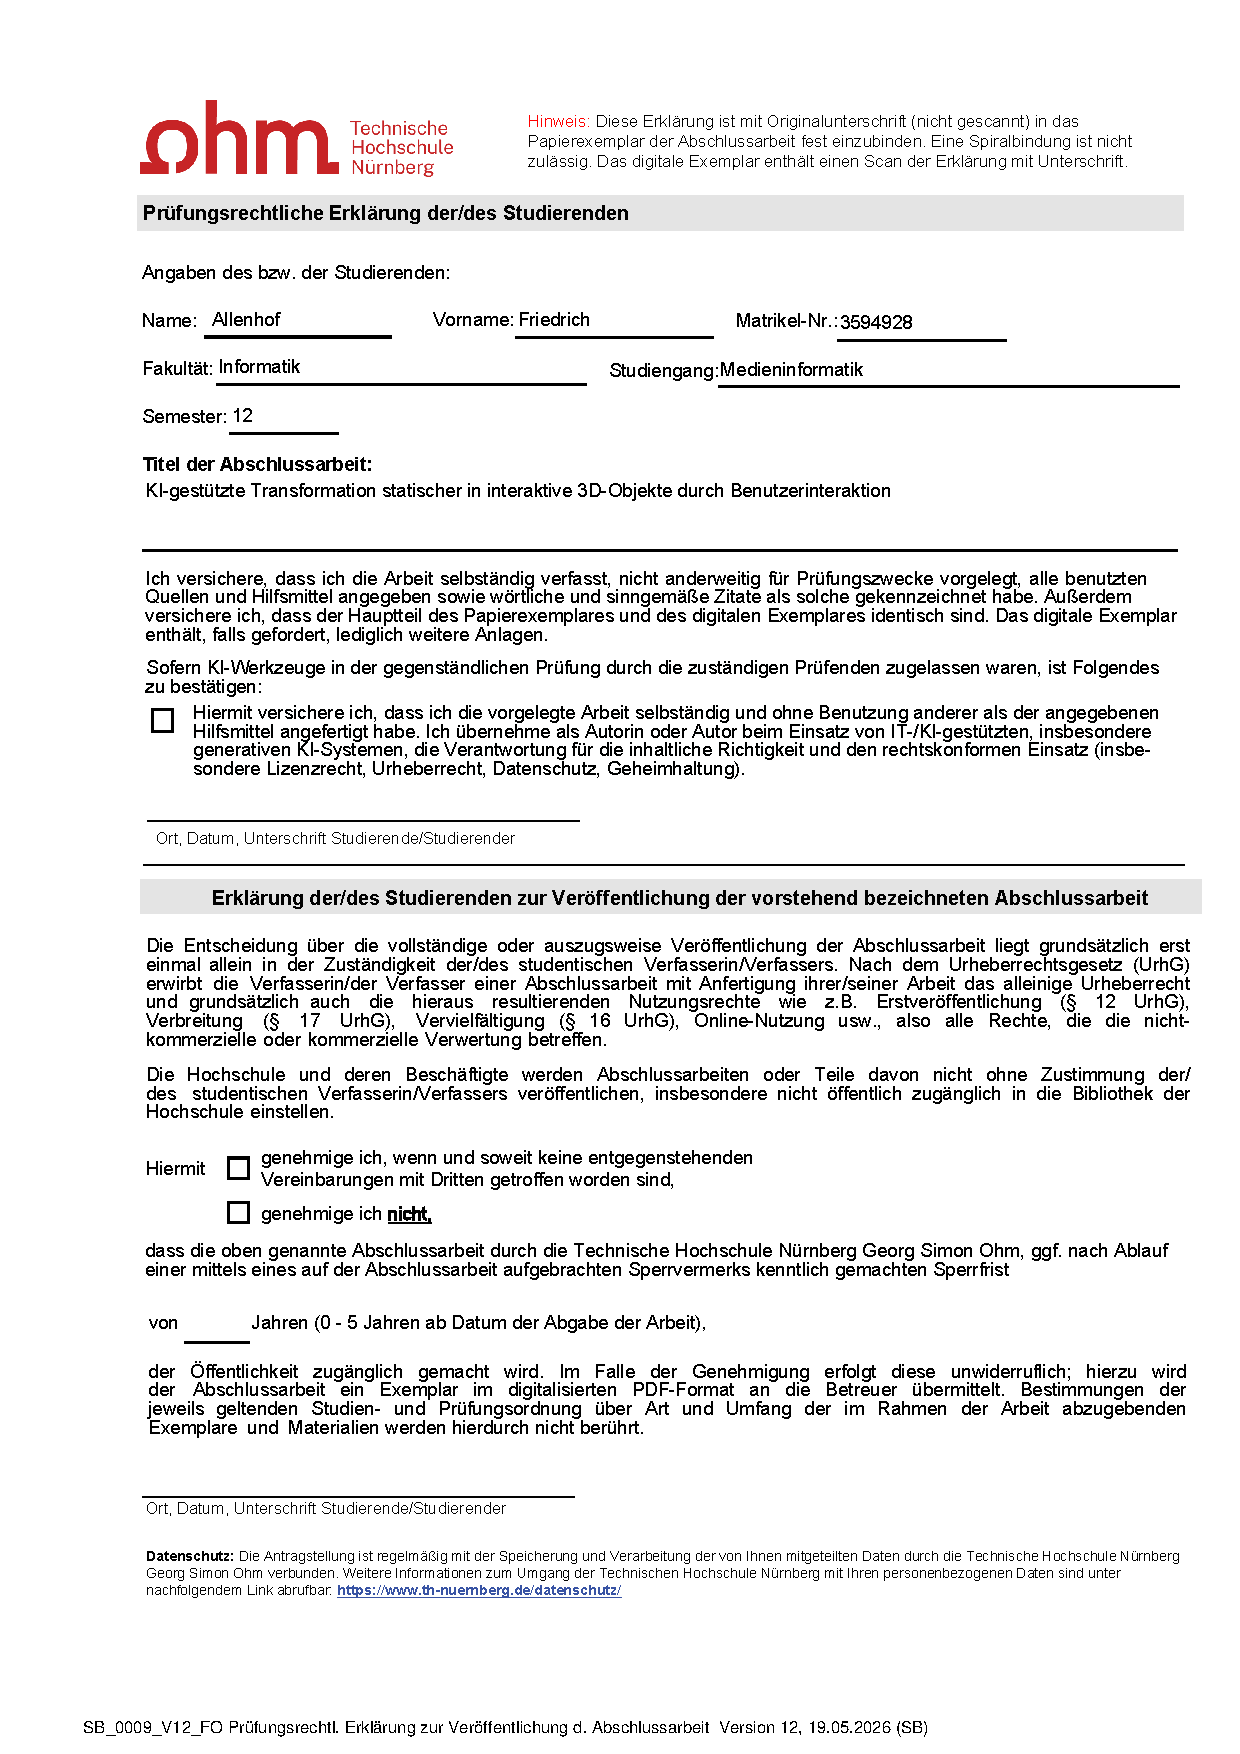
\includepdf{SB_0009_FO_Pruefungsrechtliche_Erklaerung_und_Erklaerung_zur_Veroeffentlichung_der_Abschlussarbeit_public.pdf}\cleardoublepage

\section*{Abstract}
\label{sec:abstract}
\noindent\rule{\linewidth}{0.8pt}\par\nopagebreak
\vspace{2pt}
Interaktive virtuelle Prototypen ermöglichen ein frühzeitiges Testen des Verhaltens digitaler Objekte. Vorhandene 3D-Assets enthalten vorrangig Geometrie, Transformationen und Materialien, aber keine explizite Interaktionslogik. Diese Arbeit untersucht, wie sich solche statischen 3D-Objekte mithilfe natürlicher Sprache in interaktive Prototypen überführen lassen, ohne ihre Geometrie zu ersetzen. Dafür wurde der \textit{Vivian Specification Generator} (VSG) konzipiert und prototypisch umgesetzt. Der Ansatz verwendet eine Unity-basierte Vorverarbeitung sowie eine modulare, \textit{Large Language Model} (LLM)-gestützte Pipeline bestehend aus \textit{Scene Analyzer}, \textit{Interaction Planner}, \textit{Specification Generator}, \textit{Consistency Reviewer} und \textit{Unity-Validator}. Aus strukturierten Szenendaten, gerenderten Ansichten und Nutzer*innenbeschreibungen erzeugt der VSG Vivian-kompatible Spezifikationsdateien für ein zustandsbasiertes Interaktionsverhalten. Die technische Systemevaluation anhand der Testassets Lampe, Display und Toaster mit insgesamt 60 Durchläufen zeigt, dass der VSG vorhandene 3D-Objekte grundsätzlich in interaktive Prototypen überführen kann, da 57 Spezifikationen technisch valide generiert wurden. Die implementierten Korrekturmechanismen erhöhten die technische Erfolgsquote außerdem von 88,3 auf 95,0 Prozent.
Gleichzeitig verdeutlichen die Ergebnisse, dass technische Validität nicht mit funktionaler Korrektheit gleichzusetzen ist.
\par\nopagebreak\vspace{2pt}
\noindent\rule{\linewidth}{0.8pt}

\vspace{1em}
\noindent\textbf{Schlagwörter:} Interaktive Prototypen, KI-gestützte Transformation, Virtual Prototyping, Generative KI, Large Language Models, Virtual Reality
\cleardoublepage

\tableofcontents

\mainmatter
\chapter{Einführung}\label{ch:einführung}

Bei der Betrachtung dreidimensionaler Objekte in einem virtuellen Raum lässt sich deren Funktion häufig sofort erkennen. Ein Knopf soll gedrückt werden, ein Hebel soll sich bewegen, ein Display soll Informationen anzeigen und eine Lampe soll leuchten. Diese Funktionen sind von uns Menschen oft intuitiv aus Form, Position, Material und Kontext ableitbar. In virtuellen Umgebungen gilt dies jedoch nicht automatisch, da ein 3D-Modell zwar meist eine sichtbare Form, Materialien und räumliche Eigenschaften besitzt, aber in der Regel kein Verständnis über seine mögliche Nutzung. Auch Online-Bibliotheken, mittels 3D-Scanning erfasste Modelle realer Objekte sowie generativ erzeugte Inhalte liefern in der Regel kein Wissen darüber, welche Teile bedienbar sind oder wie diese auf Nutzer*innenhandlungen reagieren sollen. Zwischen dem visuellen Erscheinungsbild eines 3D-Objekts und seinem tatsächlichen Verhalten in einer virtuellen Welt liegt damit eine Lücke (siehe Abbildung~\ref{fig:intro_asset_examples}).

\begin{figure}[htbp]
    \centering
    \begin{subfigure}[b]{0.3\linewidth}
        \centering
        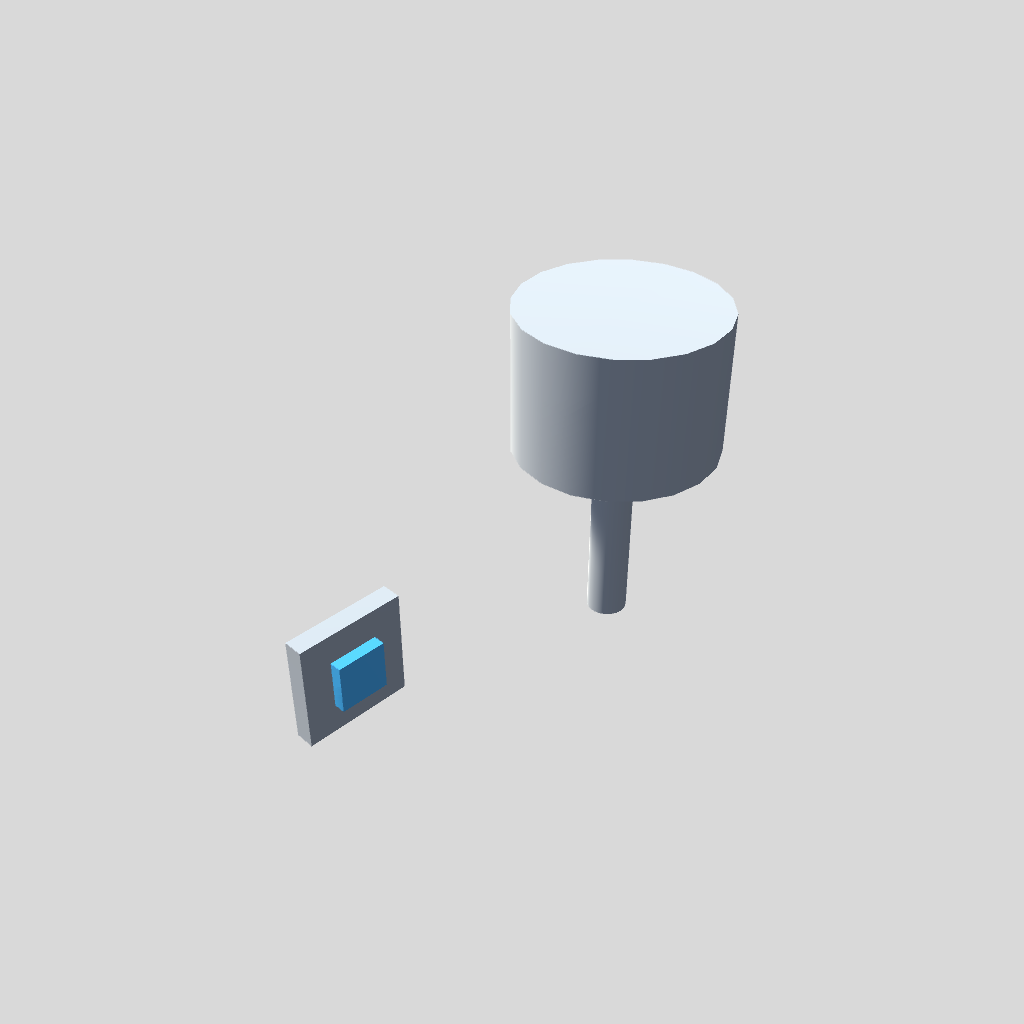
\includegraphics[width=\linewidth]{figures/asset-examples-iso/Lamp_iso_top_right}
        \caption{Lampe}
    \end{subfigure}\hfill
    \begin{subfigure}[b]{0.3\linewidth}
        \centering
        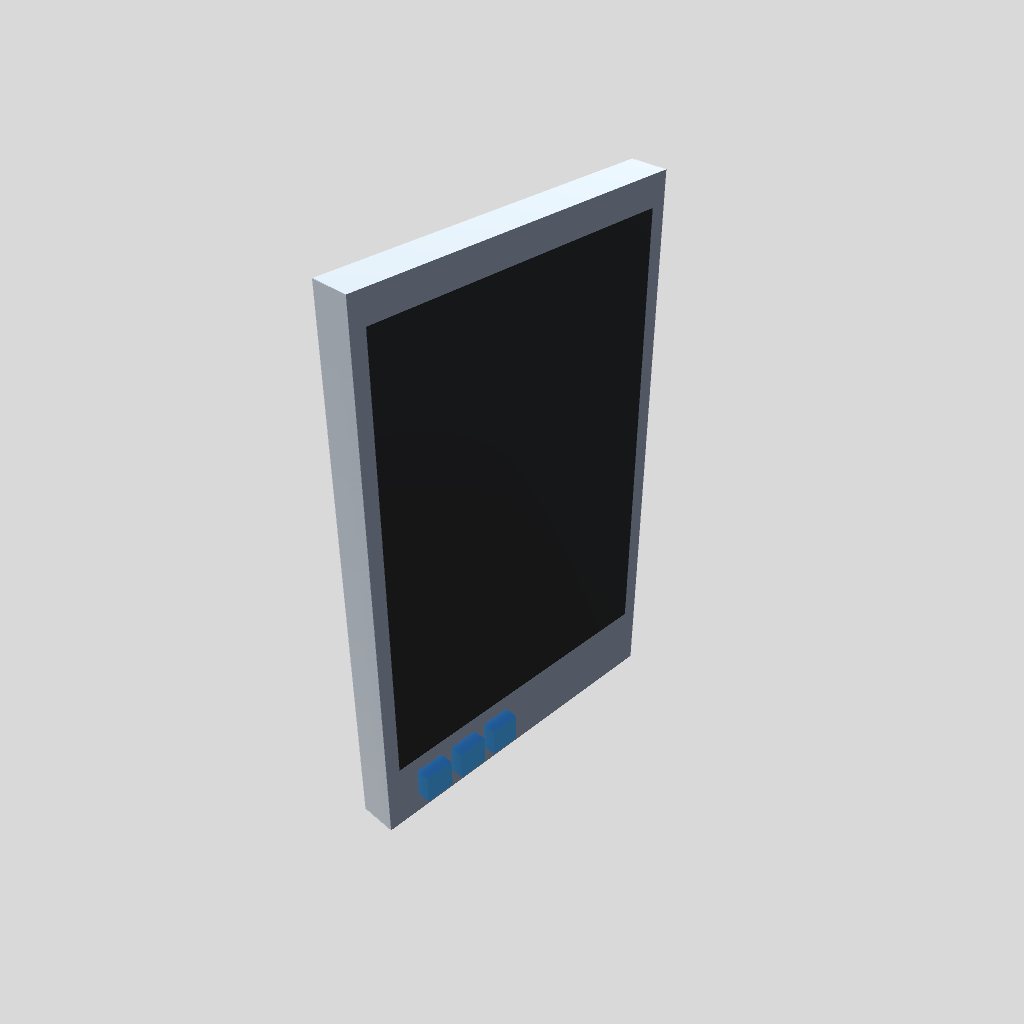
\includegraphics[width=\linewidth]{figures/asset-examples-iso/Display_iso_top_right}
        \caption{Display}
    \end{subfigure}\hfill
    \begin{subfigure}[b]{0.3\linewidth}
        \centering
        \includegraphics[width=\linewidth]{figures/asset-examples-iso/toaster3_iso_top_right}
        \caption{Toaster}
    \end{subfigure}
    \caption{Beispiele virtueller 3D-Objekte.}\label{fig:intro_asset_examples}
\end{figure}

Diese Lücke wird dann besonders deutlich, wenn 3D-Objekte nicht nur betrachtet, sondern als funktionale Prototypen mit bestimmtem Verhalten verwendet werden sollen. In Bereichen wie der Produktentwicklung, Lehre, \textit{Virtual Reality} oder \textit{Usability Engineering} reicht eine statische Darstellung häufig nicht aus, da Objekte ausprobiert, verändert und in ihrem Verhalten getestet werden sollen. Ein virtueller Prototyp muss damit weitaus mehr leisten als eine realistische Abbildung. Es muss Wissen darüber bestehen, welche Bestandteile relevant sind, welche davon bedienbar sind, welche Rückmeldungen gegeben werden und wie sich der Zustand des Objekts durch Interaktionen verändert.

Gleichzeitig ändert sich die Art und Weise, wie solche interaktiven Systeme entworfen werden können. Anstelle der rein manuellen Umsetzung durch Skripte oder systemspezifische Konfigurationen rückt mit der hohen Verfügbarkeit von KI-Systemen zunehmend natürliche Sprache in den Mittelpunkt. Diese wird somit zu einer Schnittstelle zwischen fachlicher Vorstellung und technischer Umsetzung. Der Fokus verschiebt sich von direkter Programmierung hin zur Beschreibung von Verhalten, Funktionen und Beziehungen.

Leistungsfähige \textit{Large Language Models} (LLMs) haben in den vergangenen Jahren eine rasante Entwicklung erfahren und können natürliche Eingaben interpretieren, semantische Zusammenhänge ableiten sowie strukturierte Ausgaben erzeugen~\cite{caffagniRevolutionMultimodalLarge2024,yinSurveyMultimodalLarge2024}. Dies eröffnet neue Möglichkeiten, die Lücke zwischen statischen 3D-Objekten und interaktiven Prototypen zu schließen, indem natürlichsprachliche Beschreibungen als Eingabe genutzt und mittels KI-gestützter Verfahren in eine maschinenlesbare Interaktionslogik übersetzt werden.

An dieser Stelle setzt die vorliegende Arbeit an. Sie untersucht, inwieweit sich bereits vorhandene statische 3D-Objekte in virtuellen Welten mithilfe eines KI-gestützten Workflows und natürlicher Sprache in interaktive virtuelle Prototypen überführen lassen. Als Grundlage dient das Vivian-Framework, welches Interaktion deklarativ über maschinenlesbare Spezifikationsdateien beschreibt. Damit bietet es eine geeignete Zielrepräsentation für eine automatisierte, durch Sprachmodelle gestützte Generierung.

\section{Problemstellung}\label{sec:problemstellung}

% Im Vivian Framework geschieht die Erstellung virtueller Prototypen deklarativ über Konfigurationsdateien für Interaktionselemente (InteractionElements), Visualisierungselemente (VisualizationElements), Zustände (States) und Übergänge (Transitions) in Verbindung mit einem statischen 3D-Modell. Obwohl dieses Vorgehen Interaktivität ohne tiefgreifende Programmierkenntnisse möglich macht, ist die manuelle Erstellung solcher Spezifikationen aufwendig sowie fehleranfällig. Es müssen sowohl die zulässigen Elementtypen, Attribute, Zustände, Events und Guards bekannt sein, als auch Namensreferenzen zwischen 3D-Szene und Spezifikation konsistent bleiben, da das Framework ein Verhalten über diese Referenzen an die Objekte einer 3D-Szene bindet.

% Mit steigender Komplexität eines Prototypen steigt diese Fehleranfälligkeit noch weiter. Dabei können diese syntaktischen, semantischen oder referenziellen Ursprungs sein und werden im Vivian Framework teils erst zur Laufzeit sichtbar.
% Um Spezifikationen automatisiert zu generieren, sind also formal gültige JSON-Strukturen allein nicht ausreichend. Inhaltlich plausible Interaktionen, korrekte Zustandsmodelle sowie konsistente Referenzen über mehrere Artefakte hinweg sind ebenfalls notwendig.
% Verwandte Arbeiten beschäftigen sich häufig mit Geometrie- oder Szenengenerierung, während

In der Regel enthalten statische 3D-Objekte Geometrie, Materialien und Transformationen, jedoch kein Wissen darüber, welche expliziten Teile bedienbar sind, welche Funktion sie erfüllen oder wie sie auf Nutzer*innenhandlungen reagieren. Für Interaktivität sind aber genau diese Informationen von fundamentaler Bedeutung, nämlich wenn Objekte oder Teilobjekte mit Bedeutung, möglichen Handlungen und Verhalten verbunden werden~\cite{kallmannModelingBehaviorsInteractive2002}.
Somit bestehen virtuelle, interaktive Prototypen nicht nur aus einer 3D-Geometrie, sondern besitzen zusätzlich semantisch-verhaltensbezogene Informationen.

Die Erstellung interaktiver 3D-Szenen oder die Transformation dieser in interaktive Prototypen setzt oft ein technisches Verständnis und Wissen voraus, wie etwa in 3D-Modellierung, Szenenaufbau oder Programmierung, was die Einstiegshürde für potenzielle Anwendende wie Produktentwickler*innen, Designer*innen oder Lehrende vergrößert. Diese Gruppe von Anwender*innen wird in dieser Arbeit als nicht-technische Benutzer*innen bezeichnet, also Personen ohne Kenntnisse in der Programmierung oder 3D-Modellierung. Die Fähigkeit, fachliche Anforderungen und Funktionalität präzise formulieren zu können, wird dabei jedoch vorausgesetzt.

Interaktivität wird meist an konkrete Objekte oder Teilobjekte gebunden. Verfahren wie 3D-Scanning erlauben allerdings häufig nur eine monolithische Erzeugung statischer Abbildungen der Realität. Auch rekonstruierte Szenen aus Punktwolken bieten an sich keine einzeln adressierbaren Teile. Diese Abbilder sind somit überwiegend nicht semantisch segmentiert und Objekte existieren nicht als eigenständige, adressierbare Entitäten. Eine interaktive Anpassung oder Segmentierung im Nachhinein ist dann nur mit massivem manuellem Aufwand möglich.

Weiterhin muss Interaktionsverhalten in eine konsistente, maschinenlesbare Repräsentation überführt werden, da interaktive Prototypen mehr als eine rein textuelle Beschreibung des gewünschten Verhaltens benötigen. Diese Überführung ist in der Regel ebenfalls mit hohem manuellem Aufwand verbunden und dadurch auch fehleranfällig.

Außerdem fehlen in automatisierten Verfahren zur Erstellung und Bearbeitung von virtuellen Prototypen oft interne Prüf- oder Korrekturmaßnahmen, um Fehler frühzeitig und im Prozess erkennen und beheben zu können. Diese Fehler müssen dann häufig zeitaufwendig und manuell im Nachhinein behoben werden. Auch können Halluzinationen auftreten, wie etwa in 3D-LLMs, wodurch Objekte teils nicht existieren oder falsche Beziehungen zwischen Objekten bestehen~\cite{pengUnderstandingEvaluatingHallucinations2025}.

Daraus lässt sich das zentrale Problem dieser Arbeit ableiten: Es fehlt ein niedrigschwelliger und dennoch kontrollierbarer Ansatz, mit dem bereits vorhandene statische 3D-Objekte in maschinenlesbare, validierbare und zustandsbasierte Prototypen überführt werden können, während die Geometrie beibehalten wird.


% Eine adressierte Problemstellung meiner Arbeit ist der manuelle Aufwand der Erstellung einer Vivian Spezifikation. Dies erfordert nicht nur Korrektheit der Werte sondern auch ein striktes Einhalten der benötigten Struktur.

% Eine adressierte Problemstellung meiner Arbeit ist die Planung der Einzelkomponenten, in der entschieden werden muss, welche Artefakte einer Spezifikation benötigt werden. Weiterhin muss das Wissen (Namen der Interaktionselemente, Zustände, etc.) über die einzelnen Teilartefakte zentral gespeichert werden, um darauf von verschiedenen Orten aus zuzugreifen. So kann Konsistenz der Daten über alle Artefakte hinweg gewährleistet werden.

% Da zur Erstellung einer Spezifikation für das Vivian Framework hinreichendes Wissen über dieses vorausgesetzt wird, ist ein weiteres Problem dieses Wissen einem System zu vermitteln. Es muss Kenntnis darüber besitzen, welche verschiedenen gültigen Werte und Bedingungen es für die einzelnen Artefakte zur Auswahl gibt.

% Da Fehler im Vivian Framework nativ erst zur Laufzeit geworfen werden und die Fehleranfälligkeit steigt, je komplexer das 3D-Asset ist, müssen Fehler bereits im Generierungsprozess sowie möglichst frühzeitig erkannt und abgefangen werden. Zudem ist zu berücksichtigen, ob es sich um semantische, syntaktische oder Referenzfehler handelt, damit sowohl fehlerfreie JSON-Strukturen, Gültigkeit der einzelnen Werte als auch Korrektheit der Referenzen sichergestellt werden kann. So kann außerdem ein Abbrechen des Systems verhindert werden, wenn Fehler im Generierungsprozess auftreten.


\section{Forschungsfragen und Zielsetzung}\label{sec:forschungsfragen_zielsetzung}

Um den in~\ref{sec:problemstellung} beschriebenen Problemen zu begegnen, untersucht die vorliegende Arbeit die Möglichkeit, einen Ansatz zu entwickeln, welcher die automatisierte Überführung statischer 3D-Objekte in validierte, zustandsbehaftete, interaktive Prototypen ermöglicht, der insbesondere auch nicht-technischen Benutzer*innengruppen eine Nutzung ermöglicht und die Geometrie der Teilobjekte beibehält.
Im Zentrum steht die folgende Forschungsfrage:



\begin{quote}
    \textbf{Lässt sich eine automatisierte Pipeline konzipieren und prototypisch umsetzen, die vorhandene statische 3D-Objekte mittels natürlicher Sprache in interaktive Prototypen überführt und dabei vorhandene Geometrien beibehält?}
\end{quote}

Zur detaillierten Beantwortung dieser Frage werden die folgenden untergliederten Forschungsfragen definiert:

\begin{itemize}
    \item \textbf{F1:} Lässt sich ein \textit{Co-Creation-Workflow} konzipieren und prototypisch umsetzen, in dem natürlichsprachliche Beschreibung und Korrekturschleifen die Überführung statischer 3D-Objekte in interaktive Prototypen unterstützen?
          %Kann ein Co-Creation-Workflow entworfen werden, der es auch nicht-technischen Benutzer*innengruppen ermöglicht, statische 3D-Objekte in interaktive Prototypen zu überführen?
    \item \textbf{F2:} Lassen sich relevante Objekte, Teilobjekte und semantische Rollen aus vorhandenen Szeneninformationen und Nutzer*innenbeschreibungen ableiten?
    \item \textbf{F3:} Können komplexe Interaktionslogiken aus der Kombination von bestehenden 3D-Geometrien und natürlicher Sprache extrahiert und in eine maschinenlesbare Repräsentation überführt werden?
    \item \textbf{F4:} In welchem Umfang tragen implementierte Validierungs- und Korrekturmechanismen dazu bei, aus fehlerhaften oder unvollständigen Erstgenerierungen lauffähige Vivian-Spezifikationen zu erzeugen?
          % In welchem Ausmaß reduzieren Validierungs- und Selbstkorrekturmaßnahmen syntaktische, semantische und referenzielle Fehler sowie fehlgeschlagene Unity-Validierungen im Vergleich zu einem Erstgenerierungsdurchlauf ohne Korrekturschleife?
          %Inwieweit können Validierungs- und Selbstkorrekturmechanismen bei der automatisierten Erstellung von Prototypen syntaktische, semantische und referenzielle Fehler vor der Laufzeit reduzieren?
\end{itemize}

Das Ziel dieser Arbeit ist die Konzeption und prototypische Implementierung einer KI-gestützten Pipeline, welche eine Überführung von statischen 3D-Objekten in interaktive Prototypen vornimmt und dabei natürliche Sprache entgegennimmt, um auch nicht-technischen Benutzer*innengruppen einen Zugang zu bieten. Dabei sollen die Fähigkeiten von LLMs genutzt werden und ein Co-Creation-Workflow entstehen, um einen Menschen in den Generierungsprozess einzubeziehen.

\section{Abgrenzung}\label{sec:abgrenzung}

Diese Arbeit ist in Kooperation mit dem Institut für angewandte Informatik (IFAI) der Technischen Hochschule Nürnberg Georg-Simon-Ohm entstanden. Aufgrund dieser Zusammenarbeit sowie der Expertise im Vivian Framework (siehe~\ref{sec:vivian_framework}), wurde dieses als Grundlage zur Umsetzung einer solchen Pipeline gewählt. Da dieses Framework interaktive Prototypen ausschließlich über eine maschinenlesbare Beschreibung des Verhaltens möglich macht, bietet es eine Basis, auf der LLM-gestützte Verfahren aufsetzen können.

Diese Arbeit zielt nicht darauf ab, 3D-Szenendaten oder Geometrie zu generieren. Das beinhaltet komplette 3D-Szenen sowie einzelne 3D-Objekte, wie es in einigen verwandten Arbeiten der Fall ist. Es wird ausschließlich die Spezifikationsableitung bereits vorhandener virtueller Szenen betrachtet, um virtuelle Prototypen durch Verwendung des Vivian Framework zu erschaffen.


\section{Aufbau der Arbeit}

Aufbauend auf den in Kapitel 1 genannten Problemstellungen und Forschungsfragen werden in Kapitel 2 einige theoretische Grundlagen erläutert. Dazu gehören statische und interaktive 3D-Objekte, die Transformation vorhandener 3D-Assets in interaktive Prototypen, das Vivian-Framework sowie Large Language Models und agentische Systeme. Kapitel 3 ordnet den derzeitigen Forschungsstand zur Verwendung von LLMs in virtuellen 3D-Welten ein und leitet daraus die Forschungslücke ab. Darauf aufbauend beschreibt Kapitel 4 die Anforderungen an den Vivian Specification Generator sowie Architekturentscheidungen. Kapitel 5 stellt die prototypische Implementierung der Pipeline und ihrer Module vor. In Kapitel 6 wird der entwickelte Ansatz anhand verschiedener Testassets technisch evaluiert und hinsichtlich Funktionsfähigkeit, Robustheit sowie Validierungs- und Korrekturmechanismen untersucht. Schließlich fasst Kapitel 7 die Ergebnisse der Arbeit zusammen, beantwortet die Forschungsfragen und zeigt Ansätze für mögliche weiterführende Arbeiten auf.
\chapter{Grundlagen}\label{ch:grundlagen}

%TODO text einführung

\section{Statische und interaktive 3D-Objekte}\label{sec:statische_interaktive_3d_objekte}

Im Folgenden werden statische sowie interaktive 3D-Objekte definiert und erklärt.
Die Begriffe 3D-Objekt und 3D-Asset werden in dieser Arbeit simultan verwendet. Beide beschreiben ein Element einer virtuellen Szene und können als alleinige Geometrie existieren oder Unterkomponenten bzw. Teilobjekte besitzen.

\subsection*{Statische 3D-Objekte}
In dieser Arbeit werden statische 3D-Objekte als Basisform digitaler Modelle betrachtet.
Sie sind die fundamentale Basis, auf denen komplexere Verhaltensweisen aufbauen können, jedoch wohnt ihnen mit diesen Informationen noch kein Eigenleben inne.
Statische 3D-Objekte lassen sich meist rein geometrisch beschreiben.
Die Mesh-Geometrie besteht aus Dreiecksnetzen oder Polyeder-Darstellungen, welche die Oberfläche durch polygonale Flächen, in der Regel Dreiecksnetze, deren Eckpunkte (\textit{Vertices}) und Verbindungen (\textit{Edges/Faces}) definieren~\cite{botschPolygonMeshProcessing2010}.
Weiterhin besitzen sie grafische Attribute wie Materialeigenschaften, Texturen, Transparenz und Sichtbarkeit sowie eine hierarchische Anordnung im Szenengraph, welcher ihre Position, Rotation und Skalierung organisiert~\cite{GabrielZachmannsDissertation}.

\subsection*{Interaktive 3D-Objekte}

Während statische 3D-Objekte als unbelebte geometrische Körper betrachtet werden können, zeichnen sich interaktive 3D-Objekte durch Wissen über ihre Funktionalität und die Möglichkeit zur Interaktion mit ihnen aus~\cite{kallmannModelingBehaviorsInteractive2002}.
Auf diese 3D-Objekte kann durch Eingaben (\textit{Input}) eingewirkt werden und das Objekt reagiert zustands- oder verhaltensbezogen~\cite{steuerDefiningVirtualReality1992}.
Durch diese Reaktion wird aus dem statischen 3D-Objekt ein interaktionsfähiges Element.
Es ist somit in der Lage, auf durch Benutzereingaben ausgelöste Ereignisse (\textit{Events}) zu reagieren und wird zu einem handlungsoffenen Teil der virtuellen Welt. Interaktive 3D-Objekte werden in dieser Arbeit auch als interaktive Prototypen bezeichnet. %TODO auf duch Benutzer*innen

\section{Transformation statischer in interaktive 3D-Objekte}

Die in der vorliegenden Arbeit untersuchte Transformation von statisch zu interaktiv ist keine rein geometrische oder visuelle Modifikation, sondern eine semantisch-verhaltensbezogene.
Sie macht aus einem visuellen und geometrischen Asset ein interaktives Modell, welches Informationen über sein eigenes Verhalten und die möglichen Interaktionen mit diesem beinhaltet.
Mit dem Konzept dieser \textit{Smart Objects} wird Logik direkt im Objekt gespeichert, was wiederum Dezentralisierung und Wiederverwendbarkeit ermöglicht~\cite{kallmannModelingBehaviorsInteractive2002}. Dieser Prozess umfasst verschiedene Ebenen.

Zunächst wird das statische 3D-Modell segmentiert sowie semantisch etikettiert, was sich mit dem Begriff \textit{Labeling} zusammenfassen lässt.
Dabei werden rohe Mesh-Geometrien in bedeutungsvolle Teile mit bestimmten Rollen zerlegt (\zB~der Griff einer Tasse oder die Sitzfläche eines Stuhls), sodass ein System später \enquote{versteht}, welches Teil eines 3D-Objekts für welche Interaktion relevant ist und eine Zuordnung stattfinden kann~\cite{moPartNetLargescaleBenchmark2018}\cite{hassaninVisualAffordanceFunction2021}.

Im nächsten Schritt erfolgt der Übergang von der Semantik zum Verhalten mittels Zuweisung spezifischer Interaktionsmerkmale (\textit{Interaction Features}) zu den im ersten Schritt analysierten semantischen Etiketten. Diese Merkmale beinhalten eine Beschreibung der Funktionalität sowie eine Verknüpfung mit Verhaltensplänen oder Zustandsautomaten. Diese Pläne können Zustände überprüfen oder ändern und legen das erwartete Verhalten von beteiligten Akteuren fest~\cite{kallmannModelingBehaviorsInteractive2002}.

\section{Das Vivian Framework}\label{sec:vivian_framework}

Das Vivian Framework ist ein \textit{Virtual-Prototyping-Framework}.
Es erstellt virtuelle Prototypen, also digitale, interaktive Repräsentationen physischer Objekte aus der realen Welt.
Diese Repräsentation kann \zB~in der Produktentwicklung verwendet werden, um virtuelle Prototypen von echten Produkten zu erzeugen und deren Verhalten frühzeitig zu testen, ohne dass das physische Produkt tatsächlich vorhanden sein muss.
Diese virtuellen Prototypen funktionieren spezifikationsgetrieben, sodass Verhalten nicht programmatisch, sondern deklarativ als Spezifikation geschrieben wird.
Zur Laufzeit wird diese Spezifikation dann mittels einer \textit{State-Machine}-basierten Umgebung interpretiert, um ein Interaktionsverhalten abzubilden~\cite{VivianFrameworkGitLab2021}.
Ein Vorteil einer solchen spezifikationsgetriebenen Vorgehensweise ist, dass beispielsweise Produktentwickler*innen keine Programmierkenntnisse benötigen, um virtuelle Prototypen von Produkten (\textit{Digital Twins}) zu erstellen.
So kann das Verhalten eines Produktes bereits frühzeitig und iterativ getestet werden.
Ein weiteres mögliches Einsatzgebiet ist das Usability Engineering, mit dem interaktive Systeme so gestaltet und geprüft werden, dass sie für die jeweilige Zielgruppe möglichst effektiv, effizient sowie zufriedenstellend nutzbar sind.
Dafür werden Systeme nicht erst am Ende, sondern bereits in der Entwicklung, beispielsweise mittels Prototypen, hinsichtlich Gebrauchstauglichkeit analysiert und getestet~\cite{gouldDesigningUsabilityKey1985}.

\subsection*{Vivian-Spezifikationen}

Wie bereits gezeigt, besitzen statische 3D-Objekte von sich aus keine Interaktivität (siehe~\ref{sec:statische_interaktive_3d_objekte}).
Das Vivian-Framework bildet die Brücke zwischen statischem und interaktivem 3D-Objekt über eine maschinenlesbare Beschreibung des Verhaltens bei Interaktion mit dem virtuellen Prototyp.
Die Verbindung dieser Spezifikation zu einem 3D-Objekt in der Szene wird über Namensreferenzen hergestellt. %TODO vivian framework gleiche schreibweise überall?
Ein Element in der Spezifikation referenziert demnach ein gleichnamiges 3D-Objekt oder Teilobjekt in der Szene.
Weiterhin ermöglichen Spezifikationen eine Entkopplung des Verhaltensmodells vom 3D-Objekt, sodass unterschiedliche Spezifikationen verschiedene Verhalten bei demselben 3D-Objekt ermöglichen.
Sie besteht im Wesentlichen aus vier Teilen: Interaktionselemente (\textit{Interaction Elements}), Visualisierungselemente (\textit{Visualization Elements}), Zustände (\textit{States}) und Übergänge (\textit{Transitions})~\cite{VivianFrameworkGitLab2021}.

%TODO texttt weg für elemente
\textbf{Interaktionselemente.} Hier befinden sich Elemente, welche Eingaben akzeptieren und somit Interaktion ermöglichen. Das können \ua \texttt{Buttons}, \texttt{Slider} oder \texttt{Movables} sein.

\textbf{Visualisierungselemente.} Dabei handelt es sich um Elemente, welche eine visuelle Rückmeldung geben. Typisch sind hier \texttt{Light}, \texttt{Screen} oder \texttt{Sound Source}.

\textbf{Zustände.} In diesem Teil befinden sich alle möglichen Zustände, die ein Prototyp erreichen kann. Jeder Zustand beschreibt eine bestimmte Situation, indem er Interaktions- und Visualisierungselementen Werte zuweist. Diese Zuweisung kann zudem an Bedingungen geknüpft sein.

\textbf{Übergänge.} Übergänge bestimmen, wie sich ein virtueller Prototyp von einem Zustand in einen anderen verändert. Diese Übergänge können durch Zeitüberschreitungen oder Ereignisse (Events) ausgelöst werden. Zusätzlich kann ein Übergang an eine zu erfüllende Bedingung (\textit{Guard}) geknüpft sein.


\section{Large Language Models und agentische Systeme}\label{sec:llms_and_agents}

Large Language Models (LLMs) sind tiefe neuronale Netzwerke, welche die Verarbeitung von natürlicher Sprache ermöglichen~\cite{lazerSurveyAgenticAI2026}.
Sie enthalten typischerweise Milliarden von Parametern und sind in der Lage, komplexe Aufgaben zu verstehen und zu lösen oder in Teilaufgaben zu zerlegen~\cite{bommasaniOpportunitiesRisksFoundation2022}.
Ihre Skalierbarkeit ist ein zentrales Merkmal von LLMs, denn sie zeigen mit zunehmender Modellgröße und Datenmenge qualitative Leistungssteigerungen und sogenannte emergente Fähigkeiten, wie \zB \textit{In-Context Learning}.
Während solche LLMs als Modelle zur passiven Sprachverarbeitung und -generierung verstanden werden können, besitzen sie ohne zusätzliche Werkzeuge keine eigene Handlungsfähigkeit.
Hier greift das Konzept eines LLM-basierten Agenten weiter.
Ein Agent ist eine autonome Einheit, welche in einer Umgebung agiert, Entscheidungen trifft und auch mit anderen Agenten interagieren kann~\cite{shohamAgentorientedProgramming1993}.
LLM-basierte Agenten verbinden diese klassische Idee mit den Fähigkeiten von LLMs.
Ein LLM kann hier als kognitive Kernkomponente verstanden werden und verleiht dem Agenten die Fähigkeit eigenständig und unabhängig zu analysieren, zu planen sowie Probleme zu lösen~\cite{xiRisePotentialLarge2023}.
So entsteht ein System, welches nicht nur natürliche Sprache verarbeiten kann, sondern eine eigene zielgerichtete Handlungsfähigkeit besitzt und in einer Umgebung agieren kann.
Ebenso kann es zusätzliche Komponenten wie Sensorik, API-Aufrufe oder Werkzeuge nutzen~\cite{xiRisePotentialLarge2023}.
Die universelle Schnittstelle für solche agentischen Systeme, über die formuliert, geplant und koordiniert wird, ist die natürliche Sprache~\cite{shenHuggingGPTSolvingAI2023}.

\subsection*{Multimodale LLMs}

Multimodale Large Language Models (MLLMs) sind Modelle, welche im Gegensatz zu reinen LLMs nicht nur Text, sondern zudem Informationen wie Bild, Audio oder Video empfangen (Input), verarbeiten sowie ausgeben (\textit{Output}) können.
Eine für diese Arbeit wichtige Fähigkeit ist ihr Verstehen von 2D-Bildern und daraus Schlussfolgerungen zu ziehen.
Sie basieren auf LLMs und bestehen im Wesentlichen aus drei Hauptmodulen: einem vortrainierten Encoder (\textit{Modality-Encoder}), einem LLM sowie einem Adapter (\textit{Connector}).
Der Encoder verarbeitet die multimodalen Signale vor und der Adapter bildet die Brücke zum LLM, indem er diese Signale für das LLM verständlich umwandelt.
Dieser Schritt ist nötig, da LLMs (wie in~\ref{sec:llms_and_agents} gezeigt) ausschließlich Text verarbeiten können. Somit sind MLLMs in der Lage, Text sowie weitere multimodale Inhalte gemeinsam zu verstehen und darauf zu antworten~\cite{yinSurveyMultimodalLarge2024, caffagniRevolutionMultimodalLarge2024}.
Im Vergleich zu früheren, ähnlichen Arbeiten basieren MLLMs auf LLMs mit Milliarden Parametern sowie neuen Trainingsparadigmen, wie dem \enquote{Multimodal Instruction Tuning}~\cite{liuVisualInstructionTuning}.
Damit sind eine Vielzahl von Möglichkeiten gegeben, welche mit reinen LLMs nicht oder nur eingeschränkt realisierbar wären.
Solche repräsentativen Fähigkeiten sind u.a. das Verständnis von visuell geprägten Witzen oder Memes~\cite{yangMMREACTPromptingChatGPT2023,zhuMiniGPT4EnhancingVisionLanguage2023}, räumliches bzw. koordinatenbezogenes Verständnis, das Erstellen von Website-Code basierend auf handgezeichneten Entwürfen oder Kochrezepten anhand von Bildern zubereiteter Gerichte~\cite{zhuMiniGPT4EnhancingVisionLanguage2023}.

\subsection*{Verwendung in der vorliegenden Arbeit}

In dieser Arbeit werden LLM-basierte Agenten als Steuerungseinheiten in einer Pipeline zur Spezifikationsgenerierung für das Vivian Framework verwendet.
Sie übernehmen eine zentrale Rolle in der Übersetzung von natürlicher Sprache in strukturierte, maschinenlesbare Spezifikationen.
Außerdem analysieren sie 3D-Szenen, planen mögliche Interaktionen mit einem 3D-Objekt, erzeugen Spezifikationen zur Realisierung dieser Interaktionen und validieren semantische Korrektheit der erzeugten Artefakte.






\chapter{Forschungsstand}\label{ch:stand_der_forschung}

Die aktuelle Forschung in diesem Gebiet verbindet Sprachmodelle mit 3D-Repräsentationen und zeigt, dass LLM-basierte Systeme zunehmend in der Lage sind, 3D-Szenen nicht nur mit Sprache zu beschreiben, sondern semantisch sowie räumlich zu interpretieren.
Mit der Weiterentwicklung von LLMs konnte deren Integration mit räumlichen Daten große Fortschritte erzielen und bietet so neue Möglichkeiten wie Szenenverständnis, Planung und Generierung von 3D-Welten oder Navigation in diesen.
Spätestens seit 2023 hat sich die Verbindung zwischen LLMs und 3D-Repräsentationen zu einer eigenständigen Forschungslinie entwickelt, welche 3D-Szenen nicht nur beschreiben, sondern auch für neue Methoden wie das \textit{Grounding}, Fragebeantwortung und Planungsaufgaben nutzen können~\cite{maWhenLLMsStep2025,hong3DLLMInjecting3D2023}.
Trotz dieser schnellen Entwicklung bleiben Datenknappheit, Halluzinationsrobustheit und räumliches Verständnis (Grounding) zentrale Herausforderungen aktueller Systeme~\cite{pengUnderstandingEvaluatingHallucinations2025, maWhenLLMsStep2025}.

\paragraph{3D-LLMs für 3D-Verstehen.}

In Arbeiten wie 3D-LLM und PointLLM können multimodale LLMs 3D-Daten direkt verarbeiten und nehmen dafür beispielsweise Punktwolken als Eingabe entgegen, wobei PointLLM eher objektzentriert ist. Dadurch können Aufgaben wie \textit{3D-Captioning}, 3D-Fragebeantwortung, Grounding, Dialog oder Navigation bearbeitet werden und relevante komplexere Konzepte wie räumliche Beziehungen zwischen Objekten, physikalische Eigenschaften, Raumlayouts oder Interaktionsmöglichkeiten (\textit{Affordances}) verstehen~\cite{hong3DLLMInjecting3D2023,xuPointLLMEmpoweringLarge2025}.

\paragraph{LLM-gestützte Pipelines zur Szenengenerierung und -bearbeitung.}

Parallel dazu wurden LLM-gestützte Pipelines entwickelt, in denen LLMs nicht direkt 3D-Daten verarbeiten.
Stattdessen fungieren sie als Planungs- und Steuerungseinheit, die für die Generierung und Bearbeitung ganzer 3D-Szenen genutzt werden.
Das Framework LLMR nutzt für die Generierung von interaktiven Szenen einen modularen Workflow, darunter die Module Planner, Scene Analyzer, Skill Library, Builder und Inspector. Es kann Szenenkontext analysieren und generiert anschließend Unity-kompatiblen C\#-Code, welcher durch ein Inspektionsmodul iterativ geprüft wird. Als Eingabe arbeitet das System mit einer strukturierten, für das LLM konsumierbaren JSON-Repräsentation des Szenenkontexts~\cite{delatorreLLMRRealtimePrompting2024}.
HOLODECK verfolgt einen stärker szenenzentrierten Ansatz und zerlegt die Generierung einer Szene in einzelne Schritte für Grundrisse, Materialien, Fenster und Türen, Objektauswahl sowie räumliche Anordnung.
Es dient der automatisierten Erstellung von 3D-Simulationsumgebungen im Bereich der verkörperten KI (\textit{Embodied-AI}) und platziert durch ein Constraint-basiertes Verfahren Objekte räumlich plausibel im Raum~\cite{yangHolodeckLanguageGuided2024}.

\section{Artikulation statischer 3D-Objekte}
%TODO Artikulierung ersetzen

Für die Transformation statischer in interaktive Objekte sind objekt- und szenenzentrierte Ansätze besonders relevant.
ArtLLM wandelt eine Punktwolke in eine Abfolge von \textit{Tokens} um, die vom Modell nacheinander generiert werden.
Darüber hinaus können Assets auch als Bild oder Text eingegeben werden. Wichtig ist dabei, dass diese nicht direkt in das Kernmodell eingehen, sondern vorher mit Hilfe externer Generierungsmodelle in initiale Meshes und dann in Punktwolken umgewandelt werden.
Diese Struktur definiert die Positionen der einzelnen Teile, die mechanischen Gelenke sowie deren Hierarchie.
Um Positionen und Winkel anzugeben, arbeitet es mit festen Rasterstufen statt Gleitkommazahlen.
Nachdem detailliertere Geometrie über ein Zusatzmodul hinzugefügt wurde, wird diese kinematische Struktur als URDF-Datei (\textit{Unified Robotics Description Format}) exportiert und kann so in Simulationen und virtuellen Umgebungen verwendet werden~\cite{wangArtLLMGeneratingArticulated2026}.

ArtiWorld erweitert diesen Ansatz von der Objekt- auf die Szenenebene.
Das System nimmt eine textuelle Szenenbeschreibung entgegen und identifiziert auf dieser Grundlage artikulierbare Objekte.
Anschließend erzeugt es strukturelle Beschreibungen der einzelnen Beziehungen und anschließend ebenfalls vollständige URDF-Dateien, welche an die ursprünglichen Koordinaten des starren 3D-Assets angepasst werden~\cite{yangArtiWorldLLMDrivenArticulation2025}.
Die Geometrie des Originals wird dabei nicht ersetzt, sondern um Interaktivität erweitert.
Insbesondere diese Arbeit zeigt, dass strukturelle Zwischenrepräsentationen das Reasoning verbessern.


\section{Bildbasierte Eingaben}

Eingaben basierend auf Bildern gewinnen in artikulationsbezogenen Pipelines an Bedeutung.
Einzelbilder werden aktuell in mehreren Arbeiten genutzt, um simulierbare Szenen oder artikulierbare Objekte zu generieren, wie etwa in URDFormer oder ArtLLM~\cite{chenURDFormerPipelineConstructing2024,wangArtLLMGeneratingArticulated2026}.
Dabei können Bilder sowohl isoliert, wie etwa in URDFormer, als auch zur ergänzenden Eingabe, wie in ArtLLM, verwendet werden, da diese semantische Hinweise und Informationen zu potenziellen Interaktionsmöglichkeiten bieten.
Für die vorliegende Arbeit ist dieser Befund besonders relevant.
Er zeigt die Kombination aus expliziten Raumdaten in Form von strukturellen Repräsentationen wie Punktwolken oder Szenengraphen mit Transformationen und Hierarchien einerseits sowie Bildern als visuellem Grounding andererseits.

\section{Forschungslücke}\label{sec:forschungslücke}
% und Relevanz der/für die vorliegende/n Arbeit

Die in diesem Kapitel betrachteten Arbeiten zeigen, dass LLMs und MLLMs zunehmend in 3D-bezogenen Aufgabenbereichen eingesetzt werden und viele relevante Teilansätze wie 3D-Szenenverständnis, 3D-Fragebeantwortung, 3D-Grounding, Interaktions- und Aufgabenplanung, textbasierte 3D-Verarbeitung, Szenengenerierung sowie artikulationsbezogene Objektmodellierung existieren.
So adressiert 3D-LLM \ua~3D-Captioning, 3D-Fragebeantwortung, 3D-Grounding, Dialog und Navigation~\cite{hong3DLLMInjecting3D2023}.
LLMR nutzt LLMs zur Erstellung und Modifikation interaktiver 3D-Welten zusammen mit Modulen wie Planner, Scene Analyzer, Builder und Inspector~\cite{delatorreLLMRRealtimePrompting2024}.
Holodeck erzeugt 3D-Umgebungen aus Sprache und nutzt ebenfalls LLMs \ua für Objektwahl und räumliche Layout-Constraints~\cite{yangHolodeckLanguageGuided2024}.
ArtiWorld und URDFormer adressieren artikulationsbezogene \bzw URDF-basierte Simulation und Kinematik~\cite{yangArtiWorldLLMDrivenArticulation2025,chenURDFormerPipelineConstructing2024}.
Diese Ansätze adressieren jedoch meist andere Zielartefakte als die vorliegende Arbeit und erzeugen häufig neue 3D-Geometrien, bearbeitete 3D-Assets, vollständige 3D-Szenen, Unity-Code, URDF-Dateien oder robotische Simulationsumgebungen.
Die vorliegende Arbeit ist im Gegensatz dazu nicht primär als Verfahren zur Geometrie- oder Szenengenerierung einzuordnen, sondern als semantisch-verhaltensbezogener Ansatz zur Ableitung von Interaktionsspezifikationen aus vorhandenen 3D-Szenen.

Die Forschungslücke ergibt sich damit aus der Verbindung mehrerer Aspekte.
Es sollen vorhandene statische 3D-Objekte erhalten bleiben, relevante Objekte und Teilobjekte semantisch interpretiert werden und gewünschtes Verhalten soll natürlichsprachlich beschrieben werden können.
Darüber hinaus ergibt sich aus den Randbedingungen des Vivian Frameworks, dass eine maschinenlesbare Interaktionslogik entstehen soll, welche kompatibel mit dem Vivian-Framework ist.
Da LLM-gestützte Generierungsprozesse fehlerhafte Objektverweise, inkonsistente Strukturen oder unzulässige Spezifikationselemente erzeugen können, sind zudem Validierungs- und Korrekturmaßnahmen erforderlich.
Genau diese Kombination wird im derzeitigen Stand der Forschung nicht direkt adressiert.
Die Problemstellung in Kapitel~\ref{ch:einführung} nennt bereits, dass statische 3D-Objekte zwar Geometrie, Materialien und Transformationen besitzen, es aber an Wissen über bedienbare Elemente, Funktionen und Reaktionen auf Nutzer*innenhandlungen fehlt.
Dort wird außerdem bereits ein niedrigschwelliger und kontrollierbarer Ansatz gefordert, welcher vorhandene statische 3D-Objekte in maschinenlesbare, validierbare und zustandsbasierte Prototypen überführt, während die Geometrie erhalten bleiben soll.

Aus dieser Forschungslücke sowie den Forschungsfragen F1 bis F4 (siehe~\ref{sec:forschungsfragen_zielsetzung}) folgt die Notwendigkeit für ein System, welches Szeneninformationen analysiert, Nutzer*innenbeschreibungen von Interaktionen verarbeitet und daraus relevante Objekte, Teilobjekte sowie Rollen ableitet, Vivian-kompatible Interaktionsspezifikationen erzeugt und Fehler prüft sowie gezielt korrigiert.

% Aufbauend auf den in Kapitel~\ref{ch:einführung} aufgeführten Problemstellungen und Forschungsfragen, dem Stand der Forschung sowie den in~\ref{sec:vivian_framework} beschriebenen technischen Randbedingungen des Vivian-Frameworks werden zunächst zentrale Problemfelder identifiziert, die durch das in dieser Arbeit implementierte System adressiert werden sollen.
% Wie in der Problemstellung gezeigt, besitzen statische 3D-Objekte an sich zwar geometrische und visuelle Informationen, aber keine explizite Interaktionssemantik.
% Gleichzeitig erschwert manuelles Vorgehen in der Erstellung interaktiver Prototypen nicht-technischen Nutzer*innen den Zugang zu dieser.
% Vivian setzt außerdem voraus, dass Interaktionsverhalten in eine formal korrekte, maschinenlesbare Spezifikation aus Interaktionselementen, Visualisierungselementen, Zuständen und Übergängen überführt wird.
% Da LLM-gestützte Verfahren fehleranfällig sein können~\cite{zhaoSurveyLargeLanguage2026a}, müssen syntaktische, semantische und referenzielle Fehler zudem bereits vor der Laufzeit erkannt und korrigiert werden.

% Aus diesen Überlegungen ergeben sich die Problemfelder P1-P3.
% Die Anforderungen an die in dieser Arbeit implementierte Pipeline werden im Folgenden nicht empirisch durch eine Nutzerstudie erhoben, sondern aus diesen Problemfeldern, den Forschungsfragen und den Vivian-spezifischen Rahmenbedingungen abgeleitet.

% \textbf{P1: Hohe Einstiegshürde für nicht-technische Nutzer*innen.} Die Erstellung interaktiver Prototypen setzt oft Kenntnisse in der Programmierung oder 3D-Modellierung voraus. LLMR zeigt, dass natürliche Sprache zur Erstellung und Modifikation von interaktiven 3D-Szenen genutzt werden kann, es aber zudem spezialisierter Module wie Scene Analyzer, Planner, Builder und Inspector bedarf, da ein einfaches LLM für die interaktive Szenenerstellung nicht ausreicht~\cite{delatorreLLMRRealtimePrompting2024}.

% \textbf{P2: Semantische Adressierbarkeit vorhandener 3D-Objekte und Teilobjekte.} Statische 3D-Objekte enthalten meist primär geometrische, visuelle und transformatorische Informationen und keine darüber, welche Bestandteile bedienbar sind oder welche Rolle sie in einer Interaktion besitzen. Ohne diese semantische Adressierbarkeit kann eine spätere Interaktionsbeschreibung nicht mit der vorhandenen Geometrie verknüpft werden.
% Klassische LLMs und Vision Language Models (VLMs) allein sind nicht ausreichend in der dreidimensionalen Welt verankert, um statische 3D-Objekte in einer virtuellen Welt mit solchen Informationen anzureichern~\cite{hong3DLLMInjecting3D2023}.

% \textbf{P3: Fehlererkennung und Kontrollierbarkeit LLM-gestützter Generierungsprozesse.}
% LLM-gestützte Generierungsprozesse können fehlerhafte Ausgaben erzeugen, wie nicht existierende Objektverweise oder falsche Beziehungen zwischen Objekten. 3D-LLMs können \zB erheblich von Halluzinationen betroffen sein~\cite{pengUnderstandingEvaluatingHallucinations2025}. LLMR adressiert ähnliche Probleme durch einen modularen Aufbau -- ein Inspector-Modul kontrolliert generierten Code vor der Ausführung auf mögliche Kompilierungs- und Laufzeitfehler~\cite{delatorreLLMRRealtimePrompting2024}. Daher nennt die Problemstellung dieser Arbeit explizit die Notwendigkeit interner Prüf- und Korrekturmaßnahmen, um Fehler frühzeitig sowie bereits im Prozess erkennen und beheben zu können.
\chapter{Systemkonzeption und Architekturentscheidungen}\label{ch:systemkonzeption}

Im Folgenden wird der in dieser Arbeit entwickelte Ansatz als~\textit{Vivian Specification Generator} (VSG) bezeichnet.

\section{Anforderungsanalyse}

Im Mittelpunkt steht die Analyse vorhandener Szenendaten, die Wiederverwendung vorhandener Geometrien, die Erzeugung Vivian-kompatibler Spezifikationen, die niedrigschwellige Eingabe gewünschter Interaktionen sowie die frühzeitige Erkennung und Korrektur syntaktischer, semantischer sowie referenzieller Fehler.
Zur Nachvollziehbarkeit wurden die Anforderungen in funktionale Anforderungen (A), nicht-funktionale Anforderungen (N) sowie domänenspezifische Anforderungen (D) unterteilt.

\subsection{Funktionale Anforderungen}

\begin{itemize}
    \item \textbf{A1:} Der VSG soll aus bestehenden Szenenrepräsentationen und natürlichsprachlichen Interaktionsbeschreibungen Vivian-Spezifikationsdateien erzeugen, die alle für die beschriebene Interaktion notwendigen Interaktionselemente, Visualisierungselemente, Zustände und Übergänge enthalten.
    \item \textbf{A2:} Relevante Objekte und Teilobjekte sollen vom VSG explizit identifiziert und Rollen zugeordnet werden, sodass diese eindeutig über Namensreferenzen in den Vivian-Spezifikationen referenziert werden können.
    \item \textbf{A3:} Der VSG soll erzeugte Spezifikationen syntaktisch, semantisch und referenziell prüfen. A3 operationalisiert P3.
    \item \textbf{A4:} Der VSG soll im Generierungsprozess erkannte Fehler in einem begrenzten Korrekturprozess erneut an die zuständigen Verarbeitungsschritte zurückführen. A4 adressiert erneut P3.
    \item \textbf{A5:} Um Szeneninterpretationen überprüfen und gegebenenfalls korrigieren zu können, soll ein Human-in-the-Loop-Schritt implementiert werden, um Nutzer*innen die Möglichkeit zur Prüfung und Korrektur des Interaktionsplans zu geben, bevor aus diesem eine Spezifikation erzeugt wird. Hier wird P3 adressiert und zu Teilen auch P1, da so die Kontrollierbarkeit durch Eingaben auch nicht-technischer Nutzer*innen erhöht wird.
    \item \textbf{A6:} Der VSG soll es Nutzer*innen ermöglichen, gewünschte Interaktionen natürlichsprachlich zu beschreiben, ohne dass Vivian-Spezifikationen manuell erstellt oder bearbeitet werden müssen. A6 operationalisiert P1 durch Verwendung der natürlichen Sprache.
\end{itemize}

\subsection{Nicht-funktionale Anforderungen}

\begin{itemize}
    \item \textbf{N1:} Der VSG soll einzelne Verarbeitungsschritte kapseln, sodass Zwischenartefakte separat validiert und bei Fehlern gezielt erneut erzeugt werden können.
    \item \textbf{N2:} Zwischenartefakte und Entscheidungen des VSG sollen protokolliert und abgespeichert werden, sodass der Generierungs- und Korrekturprozess nachvollzogen werden kann.
    \item \textbf{N3:} Die Implementierung des VSG soll so erweiterbar sein, dass zusätzliche Module ergänzt oder bestehende ersetzt werden können, ohne die Gesamtarchitektur grundlegend zu verändern.
\end{itemize}


\subsection{Domänenspezifische Anforderungen}
\begin{itemize}
    \item \textbf{D1:} Der VSG erzeugt Vivian-Spezifikationsdateien, welche dem von Vivian erwarteten Dateiaufbau, den erlaubten Elementtypen, den Pflichtfeldern sowie zulässigen Wertebereichen entsprechen müssen.

    \item \textbf{D2:} Der VSG darf vorhandene Geometrien und Szenenhierarchien nicht neu generieren oder ersetzen, sondern ausschließlich durch semantische und verhaltensbezogene Spezifikationen ergänzen.

    \item \textbf{D3:} Die erzeugten Bezeichner für Interaktionselemente, Visualisierungselemente, Zustände, Übergänge und Objekt-Referenzen müssen eindeutig sein.

    \item \textbf{D4:} Jede Referenz in Zuständen, Übergängen, Events, Guards und Elementdefinitionen von Interaktionselementen sowie Visualisierungselementen muss auf ein vorhandenes Szenenobjekt oder ein vorhandenes Element der Spezifikation verweisen.

    \item\textbf{D5:} Die generierte Spezifikation gilt als erfolgreich erzeugt, wenn sie in Unity mit dem Vivian Framework importiert und ohne Validierungsfehler ausgeführt werden kann.
\end{itemize}

Die Anforderungen D1-D5 ergeben sich aus der Verwendung des Vivian-Frameworks. So kann sichergestellt werden, dass Spezifikationen ausführbar erstellt werden und die gewünschte Interaktion mit einem 3D-Objekt ermöglichen.


% Wie detailliert hier den alten Ansatz erläutern?

% später ausformulieren: was macht diesen entwurf aus? Diagramm hinzufügen 
% übergang zu eigentlicher Architektur

% \begin{itemize}
% \item \textbf{Z1:} Entwicklung einer mehrstufigen Agenten-Architektur zur Zerlegung der Spezifikationsgenerierung in klar abgegrenzte Teilaufgaben.
% \item \textbf{Z2:} Entwicklung eines Systems zur automatisierten Erzeugung Vivian-kompatibler Spezifikationen aus Szenendaten und Sprache
% \item \textbf{Z3:} Integration von Validierungs- und Selbstkorrekturmechanismen zur Verbesserung syntaktischer und semantischer Konsistenz.
% \item \textbf{Z4:} Einbindung eines Human-in-the-Loop-Schritts zur Prüfung und Korrektur unklarer Szeneninterpretationen.
% \item \textbf{Z5:} Nutzer*innen sollen gewünschte Interaktionen durch Eingabe natürlicher Sprache spezifizieren können.
% \end{itemize}

% \begin{table}[h]
%     \centering
%     \caption{Übersicht der Anforderungen an den VSG}
%     \label{tab:anforderungen}
%     \begin{tabular}{ll}
%         \toprule
%         \textbf{\#} & \textbf{Anforderung} \\
%         \midrule
%         A1          & XXX                  \\
%         A2          & XXX                  \\
%         A3          & XXX                  \\
%         A4          & XXX                  \\
%         A5          & XXX                  \\
%         \midrule
%         N1          & XXX                  \\
%         N2          & XXX                  \\
%         N3          & XXX                  \\
%         \midrule
%         D1          & XXX                  \\
%         D2          & XXX                  \\
%         D3          & XXX                  \\
%         D4          & XXX                  \\
%         D5          & XXX                  \\
%         \bottomrule
%     \end{tabular}
% \end{table}
\section{Untersuchte Architekturansätze}

Im Laufe dieser Arbeit wurden verschiedene Ansätze implementiert, um das Ziel der Generierung einer vollständigen Spezifikation nach Vivian zu erreichen.
%vervollständigen: Diese werden nachfolgend aufgeführt und erklärt. welcher dann genommen wurde und grob warum

\subsection{Manager-gesteuerter Multi-Agenten-Ansatz}
%Umbenennen in "Vorgängeransatz: Manager-getriebenes Multi-Agenten-System" ?

In der ersten Iteration wurden verschiedene Multi-Agenten-Systeme angeschaut. Im Manager-Agent-getriebenen System kann ein LLM-Agent beliebig viele weitere (spezialisierte) LLM-Agenten als Werkzeuge (Tools) aufrufen, um Aufgaben von spezialisierten Agenten lösen zu lassen, welche dann ein Ergebnis zurück an den Manager liefern. Wichtig zu erwähnen bei diesem Ansatz ist, dass ein Manager Agent spezialisierte Agenten aufrufen kann, aber selbst entscheidet, ob er dies tut. Eine ähnliche Vorgehensweise ist die des dezentralisierten Systems, bei dem es allerdings keine Orchestrierungseinheit wie einen Manager gibt, sondern Agenten die Aufgabe komplett an andere Agenten abgeben können (Handoff), ohne dass diese ein Ergebnis zurück an einen Manager-Agenten liefern.
%TODO Quelle hinzufügen

Um eine übergeordnete Instanz im Prozess zu integrieren, welche sicherstellt, dass Referenzen zwischen den einzelnen Spezifikationsdateien korrekt sind und entstandene Fehler durch gezieltes Aufrufen der zuständigen spezialisierten Agenten korrigieren kann, wurde für die erste Iteration der Manager-getriebene Ansatz gewählt.
Als spezialisierte Einheiten wurden ein Szenenanalyse-Agent sowie ein Agent je Spezifikationsdatei gewählt. Weiterhin wurde ein Bestätigungsschritt implementiert, bei dem Benutzer*innen das Ergebnis des Szenenanalyse-Moduls prüfen können.

Im ersten Implementierungsdurchlauf zeigte sich, dass der Manager-getriebene Ansatz besonders bei dateiübergreifenden Referenzen und der konsistenten Benennung von Elementen zu Fehlern führte.
Da der Manager-Agent eigenständig entscheidet, welche untergeordneten Agenten er aufruft, konnten Zwischenergebnisse nicht validiert werden und Fehler sind erst am Ende des Generierungsprozesses aufgefallen.
Daher wurde dieser Ansatz zugunsten eines deterministischen modularen Workflows verworfen.

\subsection{Begründung des modularen Workflow-Ansatzes}

Die Architektur des zweiten Implementierungsdurchlaufs folgt dem Ansatz eines modularen Workflows, welcher ermöglicht, dass Module unabhängig beschrieben, validiert und erweitert werden können, ohne die Gesamtarchitektur grundlegend zu verändern (siehe N3).
Diese modulare Trennung adressiert N1 und folgt dem in~\ref{ch:stand_der_forschung} beschriebenen Ansatz von LLMR, welches ebenfalls einen modularen Aufbau verwendet~\cite{delatorreLLMRRealtimePrompting2024}.
Jedes der in Abbildung~\ref{fig:containerdiagramm_vsg} aufgeführten Module adressiert eine spezifische Teilaufgabe innerhalb des gesamten Prozesses, wodurch der Informationsfluss gesteuert werden kann und nachvollziehbar bleibt.
Der VSG besteht im Wesentlichen aus den Modulen Scene Analyzer, Interaction Planner, Specification Generator, Consistency Reviewer und Validator.

Bei einfachen LLM-Aufrufen sinkt empirisch die Regelbefolgung bei wachsender Länge und Abhängigkeit strukturierter Ausgaben, sodass halluzinierte Referenzen und unzulässige Elementtypen kaum vermeidbar wären~\cite{zhangLostintheMiddleLongTextGeneration2025}.
Ein einzelner LLM-Aufruf wäre somit nicht ausreichend -- er müsste fünf referenzierende Spezifikationsdateien gleichzeitig konsistent erzeugen und währenddessen sicherstellen, dass jeder Vivian-Elementtyp die in der Szene tatsächlich vorhandenen Unity-Komponenten besitzt.
Durch die Zerlegung in einzelne Schritte sowie den Einsatz von Zwischenvalidierungen und iterativer Fehlerbehebung ermöglicht die hier vorgestellte Pipeline die Erzeugung korrekter Spezifikationen nach Vivian.
Eine Skalierung ist durch dieses Vorgehen ebenfalls möglich: Durch Erweiterung bestehender oder Hinzufügen neuer Module könnten noch komplexere 3D-Objekte verarbeitet werden, als in dieser Arbeit betrachtet werden.
\chapter{Prototypische Implementierung der gewählten Systemarchitektur}\label{ch:konzeption_und_implementierung}
%Oder: Prototypische Implementierung des Vivian Specification Generators
In diesem Kapitel wird die Konzeption und prototypische Implementierung des Vivian Specification Generators als gewählte Systemarchitektur zur Spezifikationsgenerierung für das Vivian Framework beschrieben. Ziel war es ein System zu entwerfen, welches die theoretischen Grundlagen und Anforderungen, welche in den vergangenen Kapiteln erarbeitet wurden, in ein lauffähiges und den Anforderungen entsprechendes System umsetzt. Konkret soll dieses semantisch und strukturell korrekte Spezifikationen automatisiert erzeugen, Benutzer*innen-Feedback entgegennehmen sowie aufkommende Fehler iterativ und eigenständig beheben können.

Diese Arbeit ist in Kooperation mit dem Institut für angewandte Informatik (IFAI) der Technischen Hochschule Nürnberg Georg-Simon-Ohm entstanden. Aufgrund dieser Zusammenarbeit sowie der Expertise im \ref{sec:vivian_framework} beschriebenen Vivian Framework, wurde dieses als Grundlage zur Umsetzung einer solchen Pipeline gewählt. Da dieses Framework interaktive Prototypen ausschließlich über eine maschinenlesbare Beschreibung des Verhaltens möglich macht, bietet es eine Grundlage, auf der LLM-gestützte Verfahren aufsetzen können.

\section{Systemkontext und Schnittstellen}
%Diagramm von Mensch - Unity UI - LLM Pipeline einfügen like Koller

Im Folgenden wird ein Architekturüberblick des VSG gegeben, in dem klar abgegrenzte, spezialisierte Module mit ihrer Funktion im Prozess kurz aufgeführt werden, in welcher Reihenfolge sie aufgerufen werden und welche Informationen jeweils ein und aus gehen.

Zur Interaktion mit dem VSG wird Unity als Benutzer*innenschnittstelle genutzt.
In einem Fenster kann eine initiale Interaktionsbeschreibung eingegeben und das zu transformierende statische 3D-Asset ausgewählt werden. Durch die Verwendung vorhandener Geometrie adressiert dieser Schritt D2. Außerdem wird A6 behandelt, da hier natürlichsprachliche Beschreibungen entgegengenommen werden.
Abbildung~\ref{fig:systemkontextdiagramm_vsg} veranschaulicht Unity als Schnittstelle in der Gesamtarchitektur zwischen Benutzer*in und KI-Pipeline.

\begin{figure}[htbp]
    \centering
    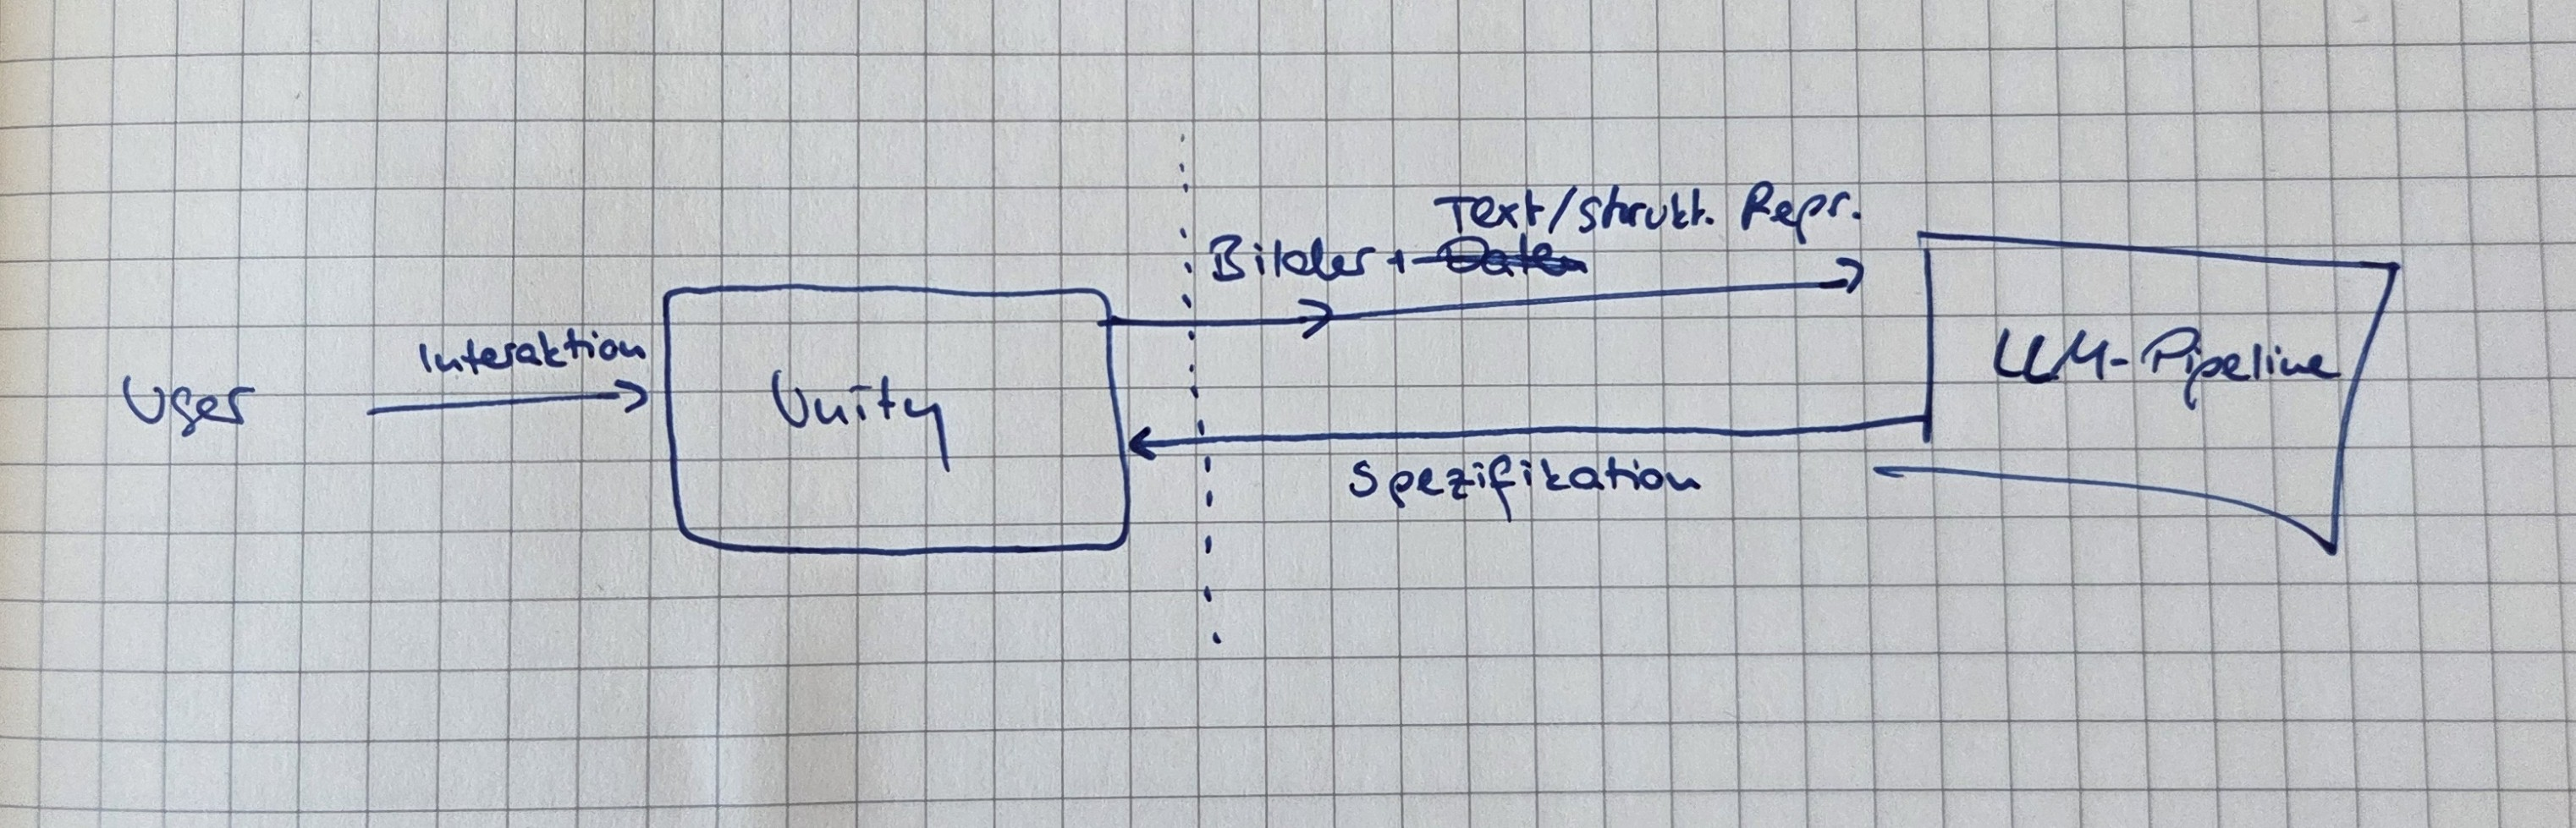
\includegraphics[width=0.8\linewidth]{figures/20260430_115502}
    \caption{Systemkontextdiagramm des VSG.}\label{fig:systemkontextdiagramm_vsg}
\end{figure}

Unity-Prozesse übersetzen das ausgewählte 3D-Objekt zudem in Formate, die von nachgelagerten Modulen und insbesondere den darin enthaltenen LLMs entgegengenommen werden können und zeigt die geplanten Interaktionen an, damit diese von Benutzer*innen bestätigt oder in einer Iterationsschleife korrigiert werden können. Dieser Human-in-the-Loop-Schritt adressiert A5.
Zusätzlich ist Unity die Umgebung, in der Vivian die Anreicherung eines statischen 3D-Assets mit Interaktionslogik über Spezifikationsdateien zur Laufzeit leistet.
Nach erfolgreicher Generierung der Vivian-Spezifikation liefert die KI-Pipeline diese zurück an Unity, damit dort Vivian zusammen mit statischem 3D-Asset und dieser Spezifikation ausgeführt werden kann.
Diese Gesamtarchitektur adressiert A1, da aus natürlichsprachlichen Eingaben und bestehenden Szenenrepräsentationen vollständige Vivian-Spezifikationen erzeugt werden.

Weiterhin erfolgt die Kommunikation der KI-Pipeline mit Unity über eine REST-API-Schnittstelle, sodass Funktionalitäten der Pipeline gegebenenfalls durch weitere Endpunkte erweiterbar bleiben.
Durch diese Entkopplung könnte die KI-Pipeline auch in einen übergeordneten Prozess integriert werden, ohne an die Unity-UI gebunden zu sein.

\section{Verwendete Sprachmodelle und Agenten}

%Technisch kannst du erwähnen, dass output_type=SceneUnderstanding die Ausgabe in eine Pydantic-Struktur zwingt. Die OpenAI-Agents-Dokumentation beschreibt, dass ein Agent über output_type statt Freitext einen bestimmten Ausgabetyp, z. B. ein Pydantic-Objekt, erzeugen kann und dabei Structured Outputs verwendet werden . Die Structured-Outputs-Dokumentation beschreibt außerdem, dass Antworten an ein vorgegebenes JSON-Schema gebunden werden können .

\section{Gesamtpipeline und Datenfluss}


\begin{figure}[htbp]
    \centering
    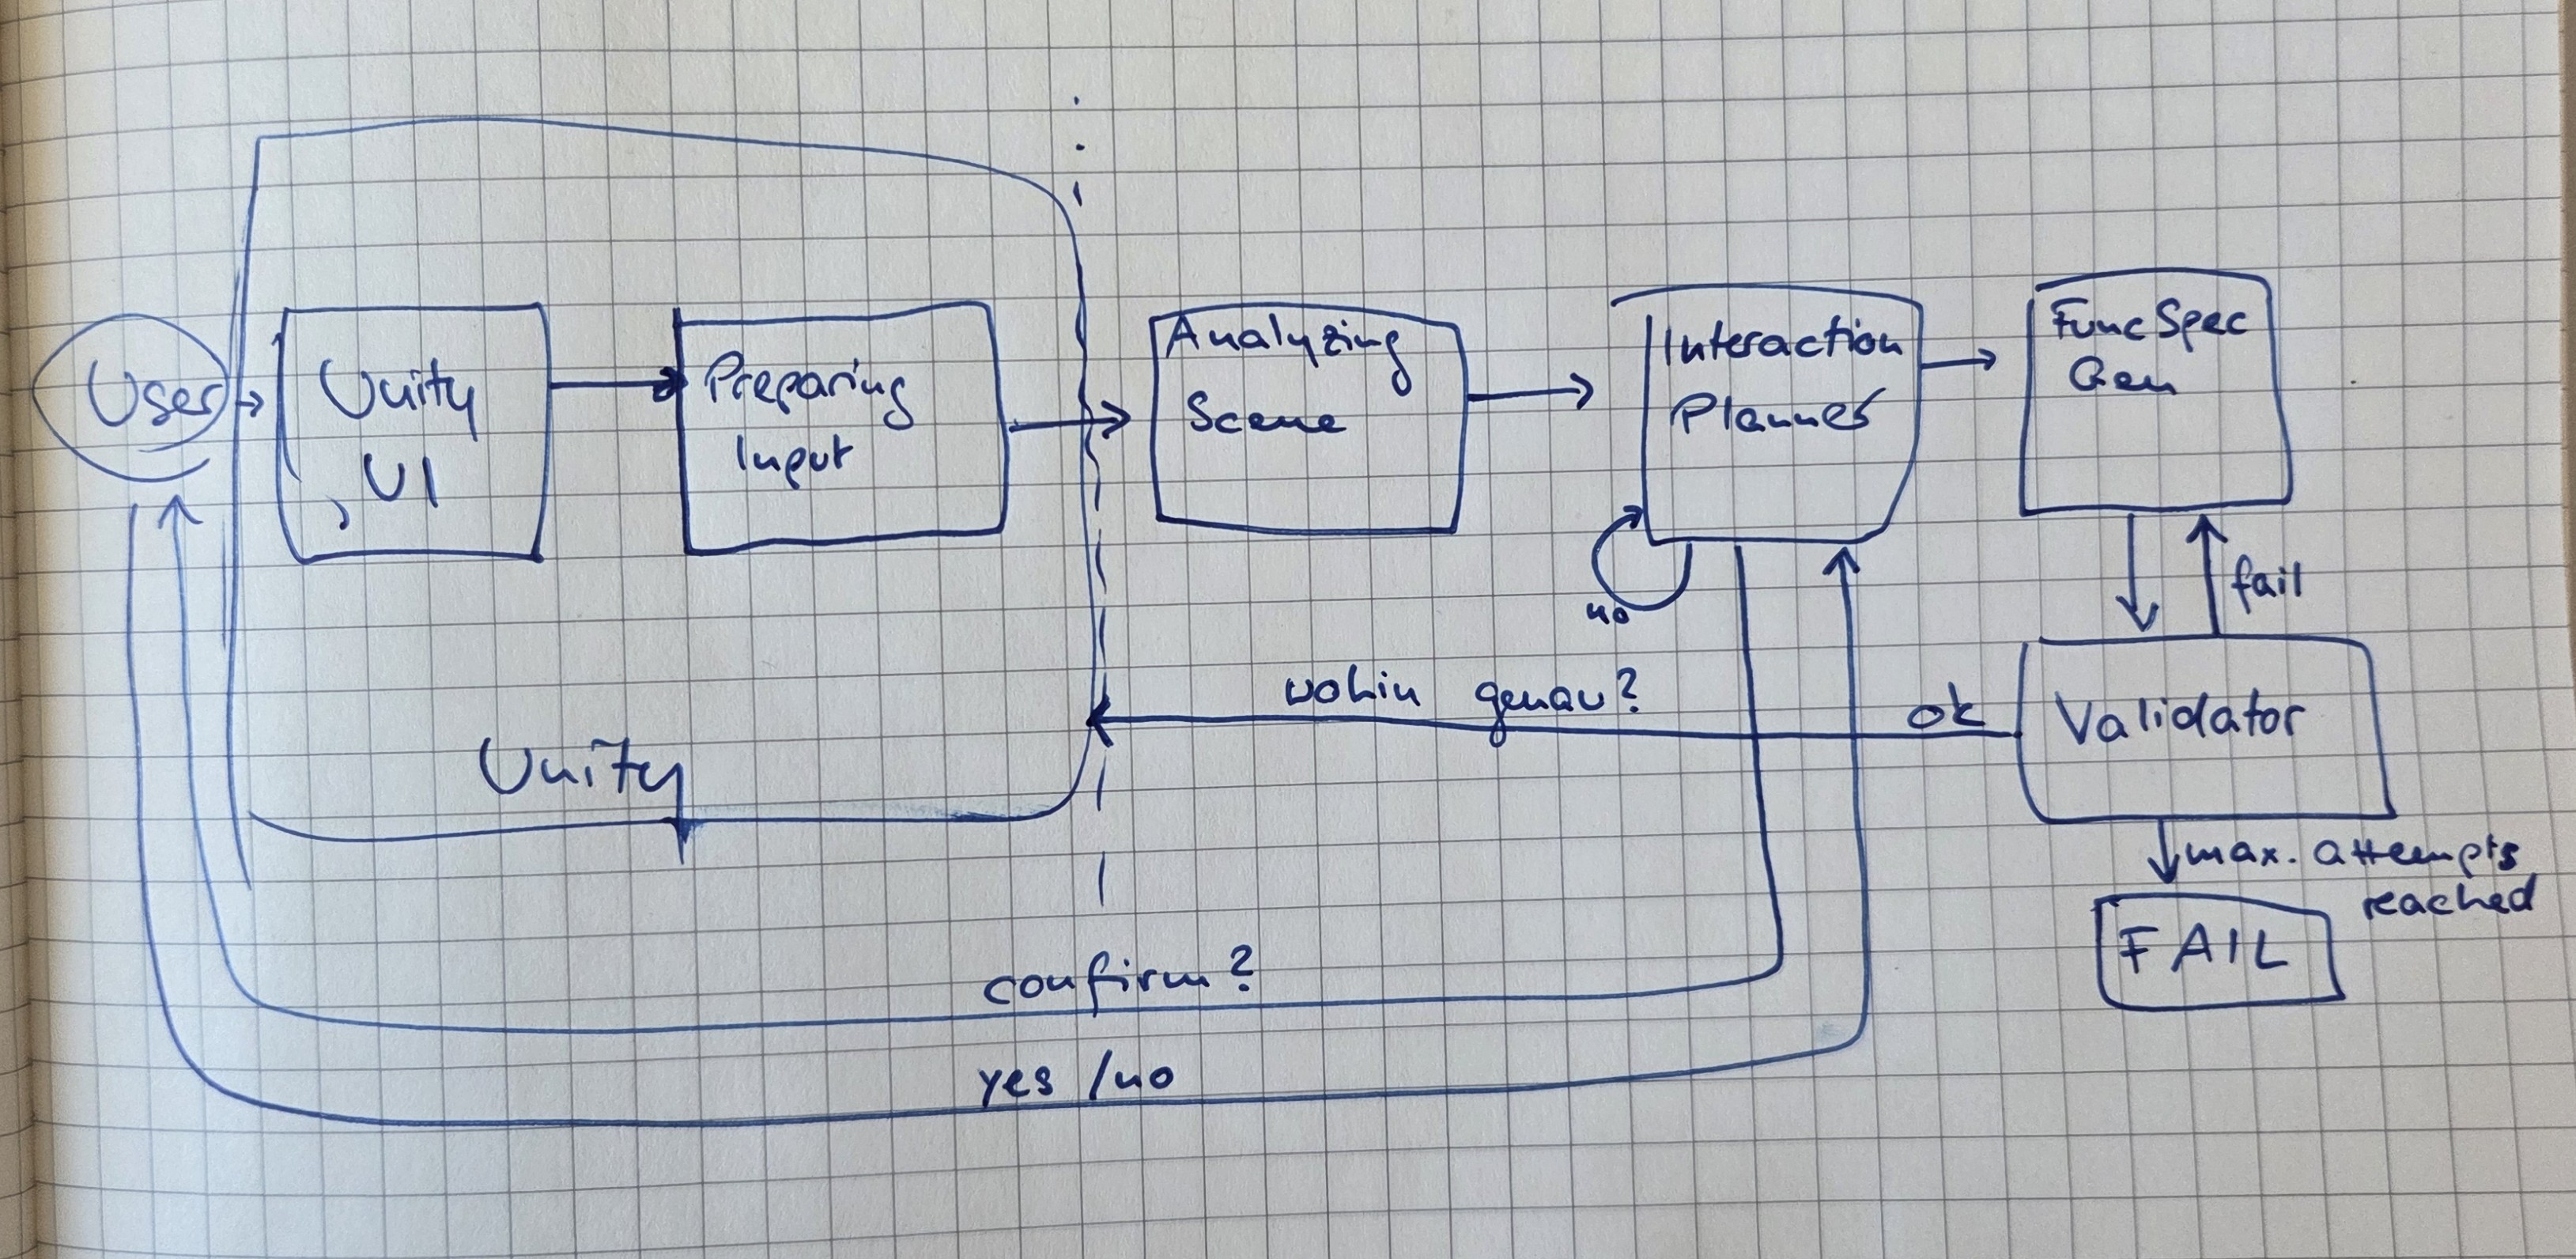
\includegraphics[width=0.8\linewidth]{figures/20260430_120448}
    \caption{Container-Diagramm des VSG.}\label{fig:containerdiagramm_vsg}
\end{figure}

Ein*e Benutzer*in kann über die Unity UI mit dem System interagieren und erhält Informationen über den Prozessfortschritt, Logging-Informationen, Rückmeldung des Interaktionsplaners und ob ein Durchlauf erfolgreich war.
Anschließend wird das ausgewählte 3D-Asset über ein weiteres Unity-Skript in eine strukturelle Szenenrepräsentation umgewandelt sowie ergänzende 2D-Bildansichten gerendert.

Diese aufbereitete Szenendarstellung wird im darauffolgenden Schritt zusammen mit einer initialen Benutzer*innenbeschreibung der gewünschten Interaktivität an den Scene Analyzer übermittelt.
Dieser gibt ein Scene-Understanding-Objekt aus, welches für jedes relevante Objekt dessen Funktion, Rolle und Eignung als potenzielles Interaktions- oder Visualisierungselement enthält.

Anschließend erhält der Interaction Planner das zuvor generierte Scene-Understanding-Objekt zusammen mit der strukturierten Szenenrepräsentation, die zuvor auch der Scene Analyzer erhalten hat, und der natürlichsprachlichen Interaktionsbeschreibung.
In diesem Schritt wird geplant, welche Interaktions- und Visualisierungselemente es geben wird, welche Zustände der Prototyp einnehmen kann und welche Übergänge zwischen Zuständen vorgesehen sind.
Der Interaction Planner gibt einen Interaction-Plan aus, welcher Element-Rollen, geplante Zustände und Übergänge sowie eine Liste der zu generierenden Spezifikationsdateien enthält.
Dieser Plan wird gemäß A5 der Benutzer*in anschließend zur Bestätigung oder Korrektur vorgelegt.
Bei einer Korrektur wird der Interaction Planner erneut aufgerufen, um diese anzuwenden, bis der Plan bestätigt wird, welcher schließlich den nachgelagerten Modulen als verbindliche Vorgabe dient.

Der Specification Generator erzeugt auf Grundlage dieses Interaktionsplans die eigentlichen Vivian-Spezifikationsdateien in der notwendigen Reihenfolge.
Ausgegeben werden vier strukturierte JSON-Dateien, welche zusammen eine Vivian-Spezifikation bilden.

Der Consistency Reviewer prüft nun mithilfe des Interaktionsplans, ob der Plan korrekt vom Specification Generator umgesetzt wurde und ob logische Widersprüche oder dateiübergreifende Inkonsistenzen existieren.
Das könnten \zB~unerreichbare Zustände oder widersprüchliche Bedingungen sein, welche eine rein strukturelle Validierung nicht erkennen kann

Ein Validator ergänzt dies um eine strukturelle und laufzeitnahe Kontrolle.
Wird die maximale Anzahl an Versuchen erreicht oder keine Fehler gefunden, terminiert der VSG.
Letzteres sorgt für ein Zurückliefern der generierten Vivian-Spezifikation an Unity, sodass Vivian diese zusammen mit dem statischen 3D-Asset ausführen kann.

% Als nächstes:
% -	Abgrenzung zu anderen systemen
% -	In-detail: was macht jedes modul und v.a. WIE funktioniert es?
% -	Fixer Agent nochmal genau überprüfen und ggf. in extra absatz, wenn der tatsächlich ne tragende rolle spielt? Und wird fixer agent auch ausgeführt, wenn Consisttency reviewer fehler erkennt?
% - unity ui einbinden

% Dann schreib einen einzigen Absatz (ca. 150–200 Wörter) zu einem Modul deiner Wahl – das, das du am besten verstanden hast. Stichpunktartig genügt: Eingabe, Ausgabe, welches Modell/welche Strategie, welche Anforderung das adressiert. Du formulierst's danach aus.


%A3/A4 Validierung + self-correction funktionieren ohne klare grenzen zwischen modulen nicht sinnvoll
%Nicht erklären WIE jedes modul intern funktioniert, das gehört in modulabschnitte

% Ein Absatz Datenfluss von Eingabe bis Ausgabe: was geht rein (Szenenrepräsentation + natürlichsprachliche Beschreibung), was passiert in welcher Reihenfolge, was kommt raus (Vivian-Spec). Hier nennst du die Module beim Namen und sagst in einem Satz, was jedes tut – aber noch keine Details, das kommt in den späteren Modulabschnitten. Lieber drei Sätze pro Modul als zehn.

% Zwischenartefakte und Kontrollfluss: welche Daten zwischen den Modulen wandern (Szenenanalyse-Ergebnis, Interaktionsplan, Spezifikationsentwurf, Validierungsbericht), wo die Validierungs-Gates sitzen (vor und nach Generierung), und wo der HITL-Schritt eingreift (vor Spec-Generierung, gemäß A5). Das ist der Absatz, der dein Diagramm in Worte übersetzt.

% Ein Absatz Abgrenzung: kurzer Vergleich zu LLMR / HOLODECK / ArtiWorld – jeweils zwei Sätze, was übernommen wird (z. B. modulare Inspection von LLMR), was bewusst anders ist (du erzeugst keine Geometrie, du fügst Verhaltens-Spezifikationen zu vorhandenen Szenen hinzu). Damit verteidigst du implizit deinen Beitrag.

% REST API -> WIE kommuniziert unity mit ki-pipeline? 


% welches sprachmodell für welches modul? klein bis groß

\section{Vorverarbeitung in Unity}\label{sec:vorverarbeitung_unity}


%TODO warum überhaupt vorverarbeiten?
Um ein 3D-Asset in MLLM-verständliche Daten umzuwandeln, müssen eine strukturelle Repräsentation und Ansichten aus verschiedenen Blickwinkeln erstellt werden.
Da der nachgelagerte Scene Analyzer mit Text und Bild als Eingaben arbeitet, benötigt er die erstellten Ansichten als visuelles Grounding für die abstrakten JSON-Daten.
Die Form des Objekts, das Material oder auch räumliche Anordnung werden somit direkt sichtbar und müssen nicht aus Bounding-Boxen rekonstruiert werden.

Im ersten Schritt wird dazu aus dem im Unity-Fenster (Abbildung~\ref{fig:unity_ui_empty}) ausgewählten 3D-Asset ein \textit{Prefab}-Objekt erzeugt, welches später von Vivian zur Laufzeit instanziiert wird.
Damit wird gemäß D2 keine neue Geometrie generiert, sondern wiederverwendet.

\begin{figure}[htbp]
    \centering
    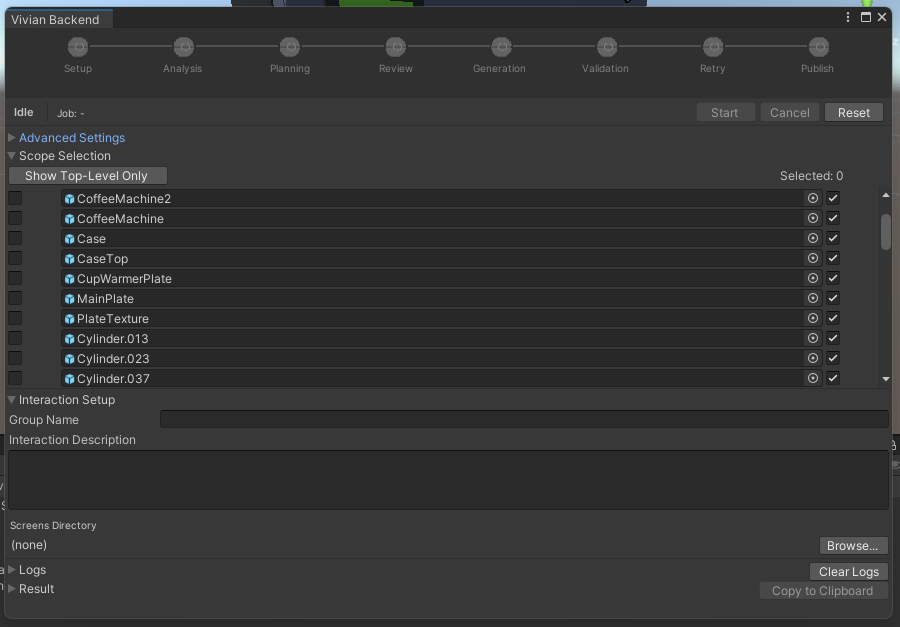
\includegraphics[width=0.8\linewidth]{figures/unity-ui}
    \caption{Unity UI des VSG.}\label{fig:unity_ui_empty}
\end{figure}

Um einem LLM Verständnis über ein 3D-Asset (in Unity\glqq GameObject\grqq{} genannt) zu geben wird zunächst eine strukturierte Szenenbeschreibung im JSON-Format mit dem Namen \textit{scene.json} erzeugt.
Dazu wird die Hierarchie des Szenengraphen rekursiv traversiert und pro GameObject Informationen wie die ID, der Hierarchiepfad, Transformation, Materialien, Bounding Boxes oder Mesh-Statistiken extrahiert.
Weiterhin werden bereits basierend auf Namen, Tags oder Material-Hinweisen heuristisch Rollen erkannt, welche im späteren Verlauf verwendet werden können, um Interaktionselemente und Visualisierungselemente zu klassifizieren.

Im Anschluss daran rendert Unity für das übergeordnete GameObject verschiedene Ansichten, da die Erkennungsleistung eines MLLM steigt, wenn statt einer Einzelansicht mehrere gerenderte Ansichten eines 3D-Objekts verwendet werden~\cite{suMultiviewConvolutionalNeural2015}.
Dafür werden sechs orthografische Ansichten entlang der Hauptachsen sowie zwei isometrische (von schräg oben) als 1024x1024-Pixel-PNGs erstellt (siehe Abbildung~\ref{fig:toaster_views}).
Die gewählte Anzahl der Ansichten ist ein Kompromiss zwischen Erkennungsrobustheit und minimal notwendigem Bildumfang, um Kosten pro Durchlauf zu sparen.
Die orthografischen Ansichten vermeiden perspektivische Verzerrung und beinhalten saubere Silhouetten, während die isometrischen Ansichten die räumliche Gesamtform und Lesbarkeit verbessern sowie drei Raumdimensionen in einer Darstellung erfassbar machen.
Zur Laufzeit wird dazu eine Kamera angelegt, anhand der Welt-Bounding-Box des Objekts platziert und auf das Objektzentrum ausgerichtet.
Alle dafür benötigten Ressourcen werden anschließend wieder freigegeben.

\begin{figure}[htbp]
    \centering
    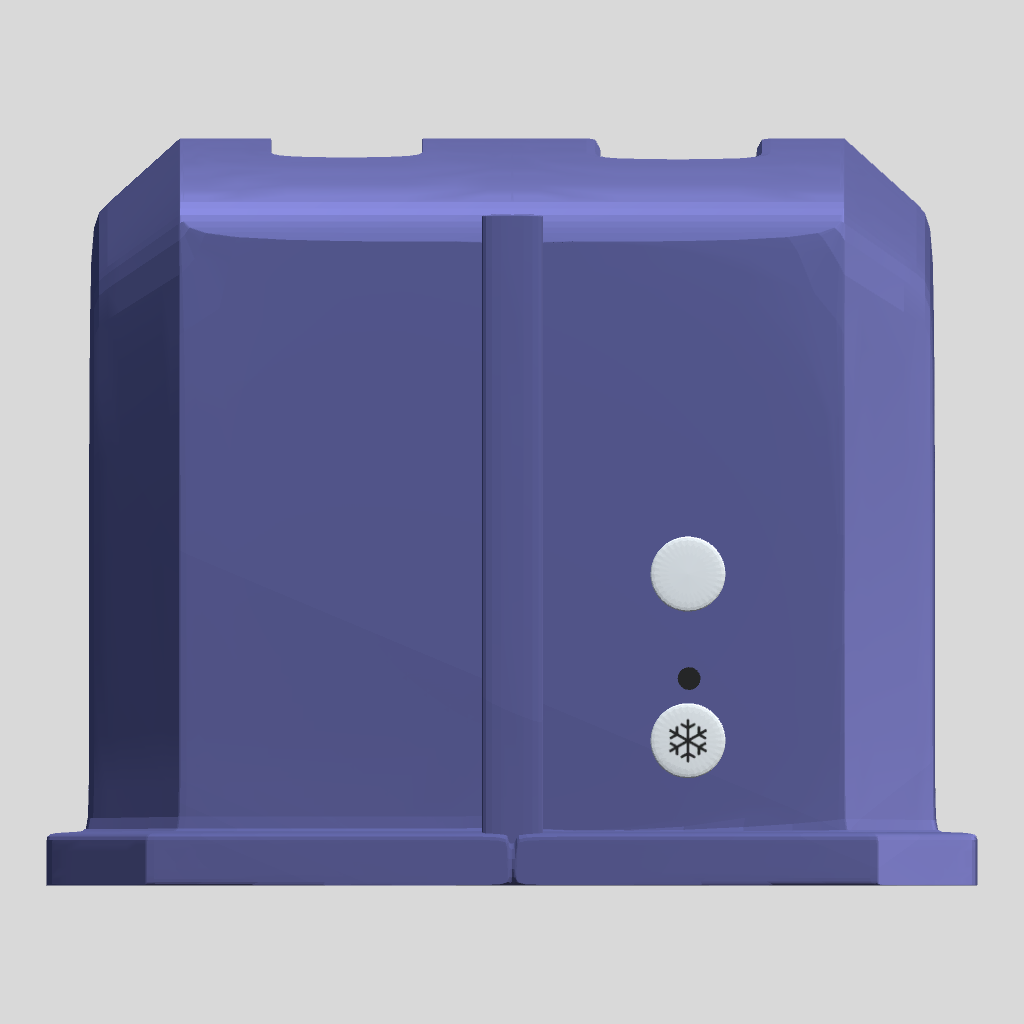
\includegraphics[width=0.22\linewidth]{figures/toaster_views/toaster3_front}\hfill
    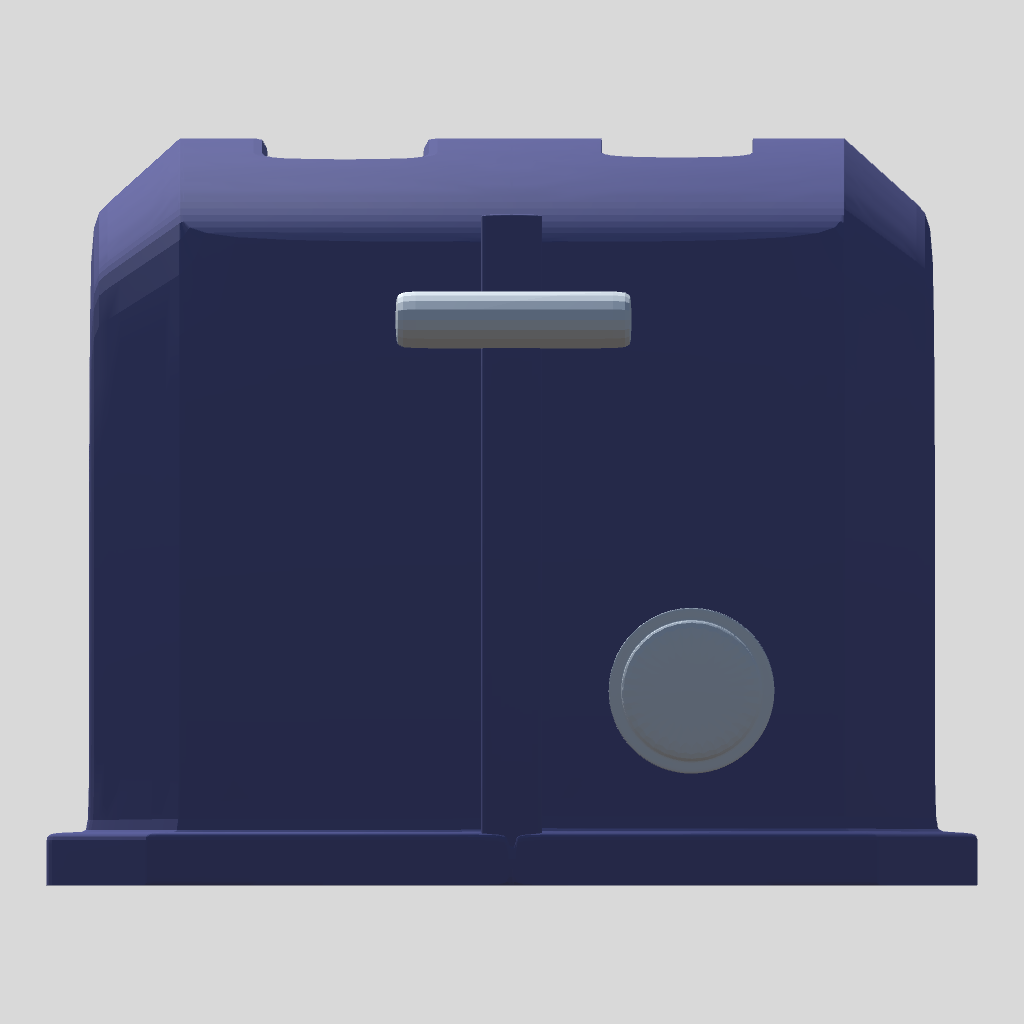
\includegraphics[width=0.22\linewidth]{figures/toaster_views/toaster3_back}\hfill
    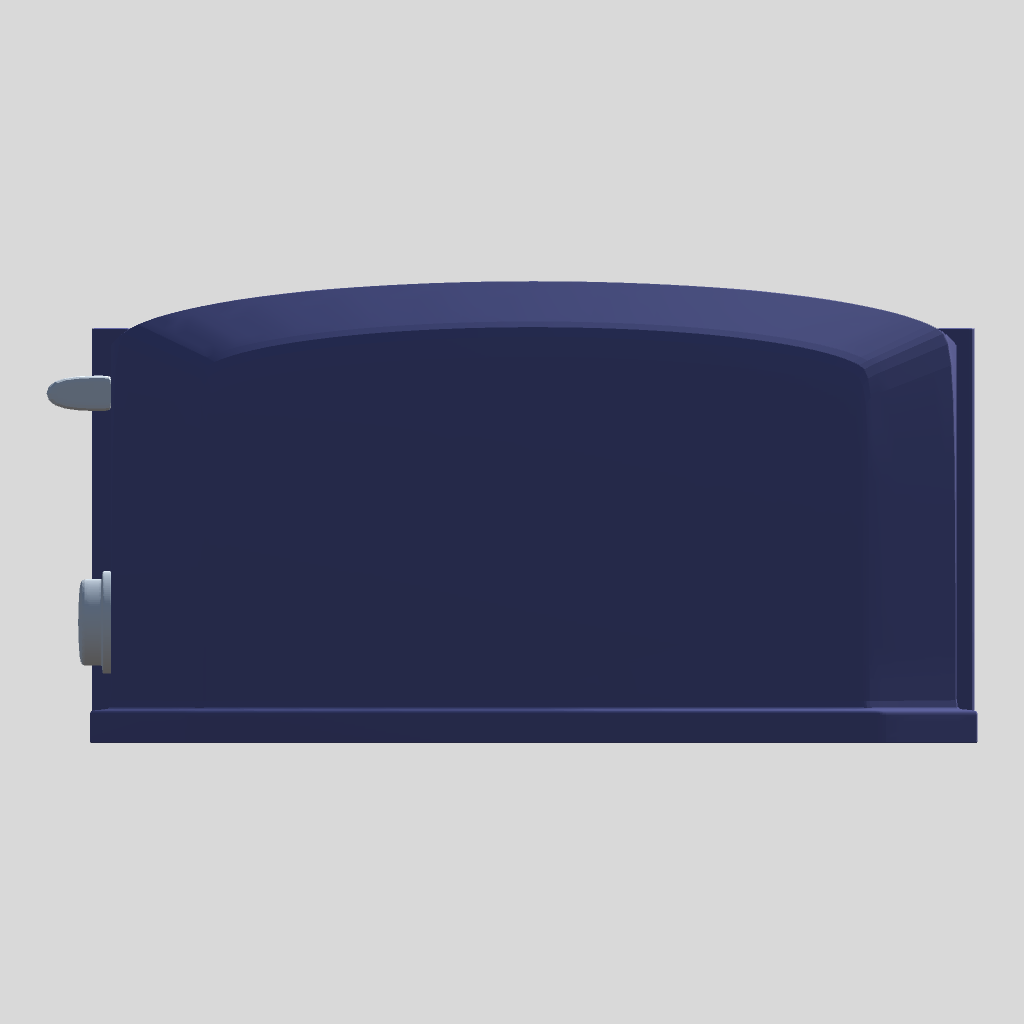
\includegraphics[width=0.22\linewidth]{figures/toaster_views/toaster3_left}\hfill
    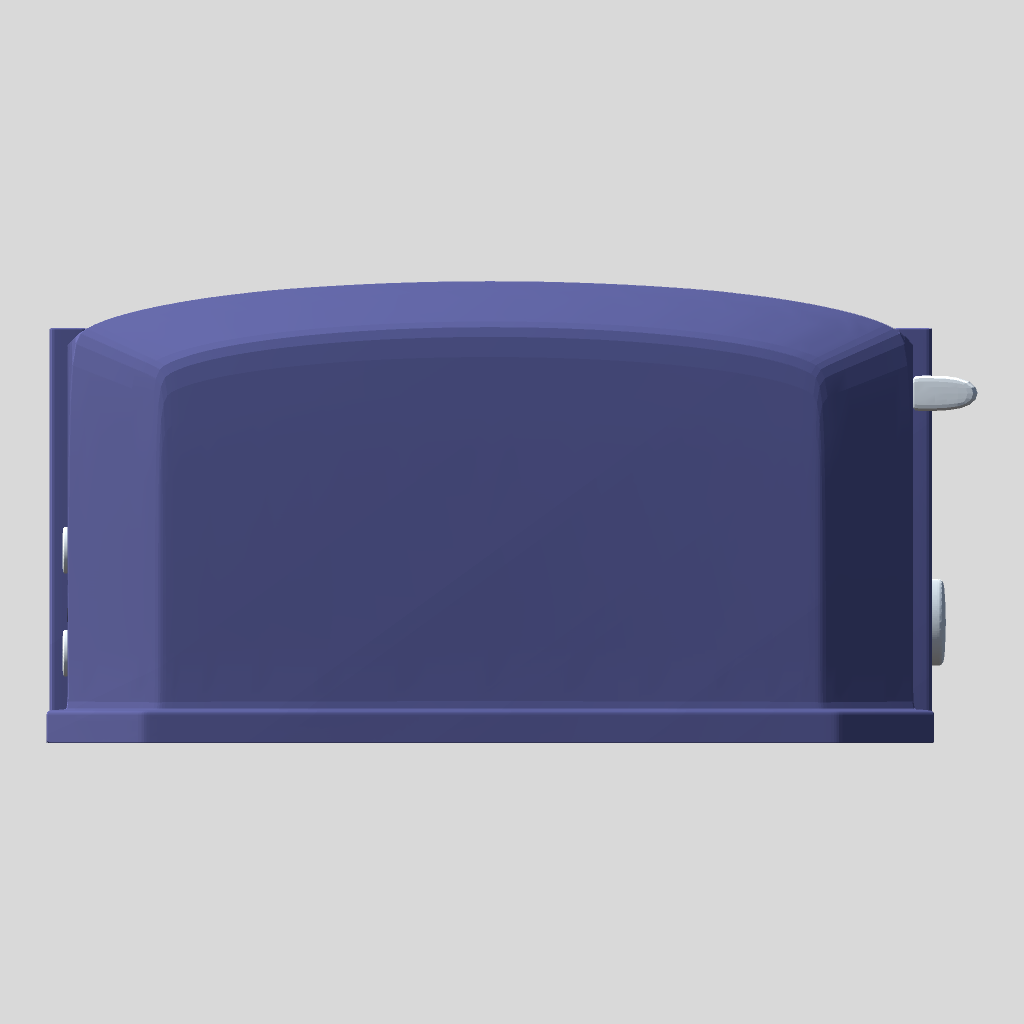
\includegraphics[width=0.22\linewidth]{figures/toaster_views/toaster3_right}\\[1em]
    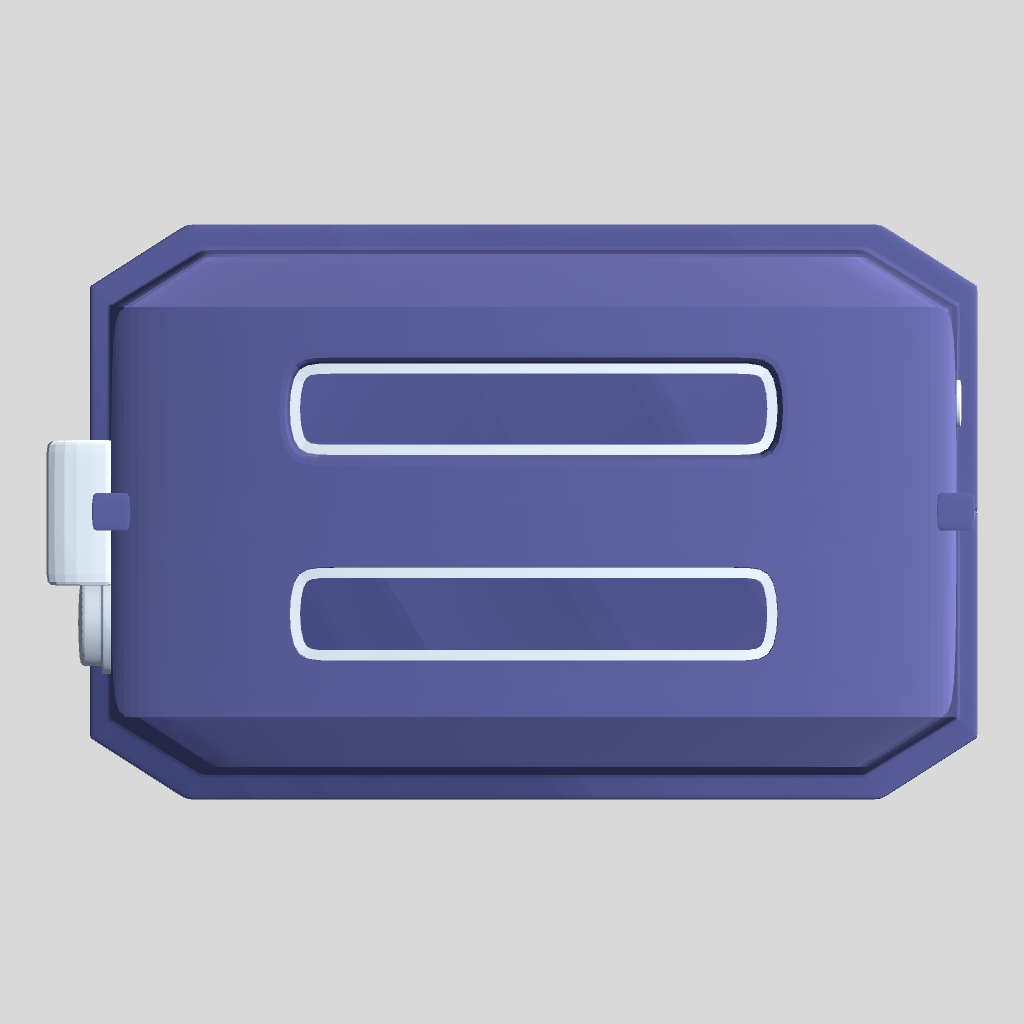
\includegraphics[width=0.22\linewidth]{figures/toaster_views/toaster3_top}\hfill
    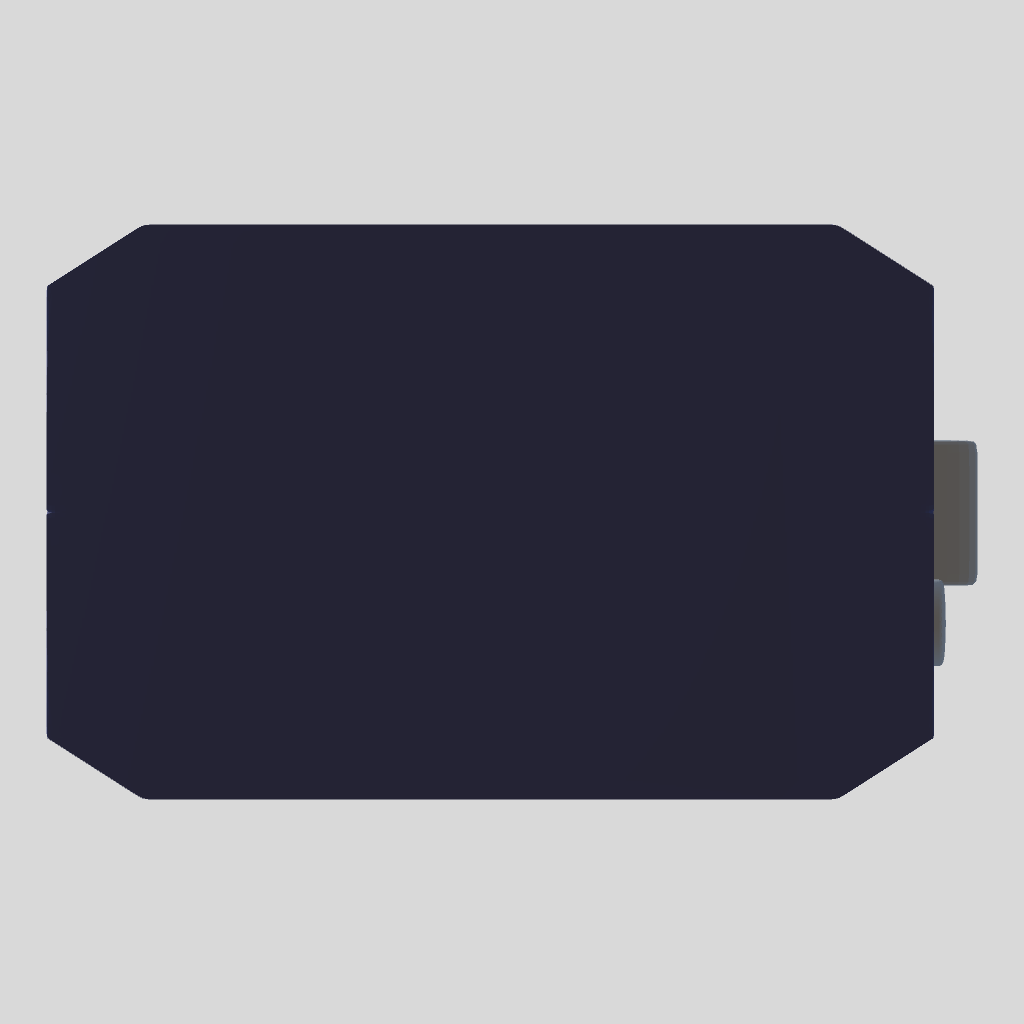
\includegraphics[width=0.22\linewidth]{figures/toaster_views/toaster3_bottom}\hfill
    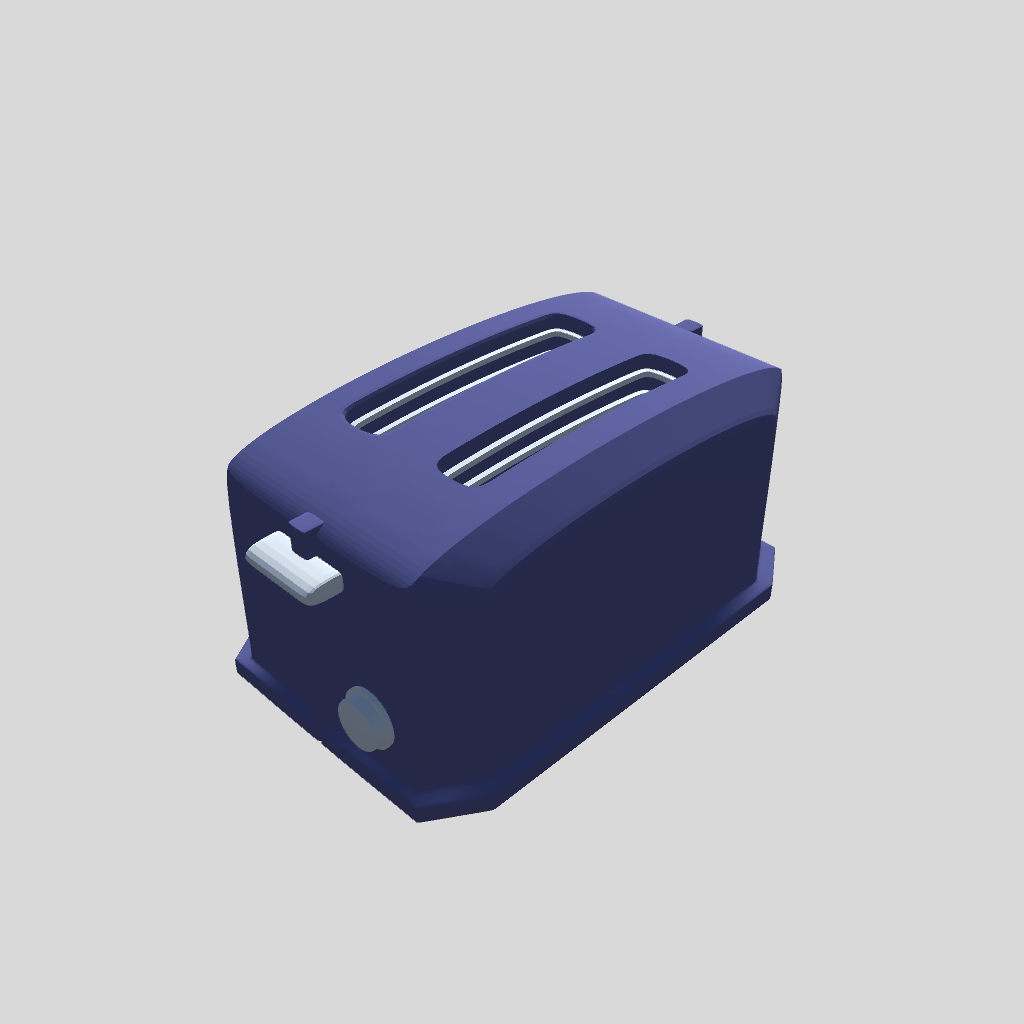
\includegraphics[width=0.22\linewidth]{figures/toaster_views/toaster3_iso_top_left}\hfill
    \includegraphics[width=0.22\linewidth]{figures/toaster_views/toaster3_iso_top_right}
    \caption{Acht gerenderte Ansichten eines Toaster-3D-Assets.}\label{fig:toaster_views}
\end{figure}

Eine zugehörige Datei namens \textit{views\_manifest.json} enthält pro Bild Kameramatrizen, Pose, Projektionstyp und einen Vermerk, welches Teilobjekt des Szenengraphen sich an welcher Stelle in der Ansicht befindet.
Unity kennt die Kameraposition die 3D-Box jedes Objekts in der Szene und kann so ausrechnen, wo sich ein Objekt der Szene im jeweiligen Bild befindet.
Nachgelagerte MLLMs können so den Zusammenhang zwischen Objekten in \textit{scene.json} und denen aus den Ansichten (siehe Abbildung~\ref{fig:toaster_views}) herstellen.
Dafür wird die ID, ein Tiefenhinweis und das Pixelrechteck vermerkt, in dem sich das Objekt im Bild befindet.

Der Vorverarbeitungsschritt in Unity erzeugt also zusammengefasst aus einem vorhandenen, statischen 3D-Asset eine strukturelle Repräsentation als JSON-Struktur, acht gerenderte Ansichten von diesem sowie eine weitere JSON-Struktur mit Informationen zu den Ansichten.
Diese Daten können nun vom nächsten Modul, dem Scene Analyzer, konsumiert werden.
In diesem Schritt werden D2, D4 sowie N1 adressiert, da Geometrie erhalten bleibt, die JSON-Struktur eine Basis für spätere Namensreferenzen bietet und definierte Ein- und Ausgabeformate verwendet werden.

% \subsection{Modul Beispiel}
% Das Modul zur Interaktionsableitung übersetzt die semantische Beschreibung eines statischen 3D-Assets in eine strukturierte Beschreibung möglicher Interaktionen. Es adressiert insbesondere die Anforderungen A2, A4 und A6. A2 fordert die Identifikation potenziell interaktiver Teilobjekte, A4 die Ableitung geeigneter Zustände und Transitionen und A6 die Ausgabe in einem maschinenlesbaren Format.

% Konzeptionell wurde das Modul als Zwischenschritt zwischen Szenenanalyse und Spezifikationsgenerierung entworfen. Dadurch wird vermieden, dass die finale Vivian-Spezifikation direkt aus unstrukturierten Eingabedaten erzeugt wird. Stattdessen entsteht zunächst eine abstrakte Interaktionsbeschreibung, die unabhängig vom konkreten Ausgabeformat geprüft und weiterverarbeitet werden kann.

% Implementiert wurde das Modul durch eine LLM-gestützte Analyse der Objektstruktur. Als Eingabe erhält es die extrahierte Hierarchie des Unity-Modells, begleitende Objektinformationen sowie die natürlichsprachliche Nutzerbeschreibung. Die Ausgabe besteht aus einer strukturierten Liste potenzieller Interaktionselemente, Zustände und Übergänge, die anschließend vom Spezifikationsgenerator in die benötigten JSON-Dateien überführt wird.

% Module:
% | Bestandteil                 | Inhalt                                                  |
% | --------------------------- | ------------------------------------------------------- |
% | Zweck des Moduls            | Welche Aufgabe übernimmt das Modul in der Pipeline?     |
% | Zugeordnete Anforderungen   | Welche Anforderungen werden durch das Modul adressiert? |
% | Konzeptionelle Entscheidung | Warum wurde das Modul so entworfen?                     |
% | Implementierung             | Wie wurde es technisch umgesetzt?                       |
% | Eingabe / Ausgabe           | Welche Daten erhält und erzeugt das Modul?              |
% | Grenzen                     | Was leistet das Modul bewusst nicht?                    |

\section{Scene Analyzer}

%noch genauer auf LLM prompt eingehen

Die Kernaufgabe des Scene-Analyzer-Moduls besteht darin, die in der Vorverarbeitung entstandenen visuellen Eindrücke und strukturellen Daten mit der natürlichsprachlichen Nutzer*innenbeschreibung zu verknüpfen und die rohen Daten so in ein semantisch angereichertes Zwischenformat zu überführen. F2 wird hier adressiert, da relevante Objekte und Teilobjekte aus Szeneninformationen und der Beschreibung abgeleitet werden, sodass nachfolgende Schritte auf diese referenzieren können.

Als Eingaben bekommt der Scene Analyzer die in Abschnitt~\ref{sec:vorverarbeitung_unity} beschriebene strukturierte Szenenrepräsentation und die Ansichten des Objekts.
Die JSON-Struktur stellt Namen, Pfade, IDs und Geometrie bereit, während die Bilder bei der semantischen Einordnung helfen.
Diese Daten werden von einem internen LLM-basierten Agenten verarbeitet, welcher so einordnen kann, ob ein Teilobjekt beispielsweise eher Griff, Display oder Knopf ist.

Das verwendete LLM leistet in diesem Modul die Hauptarbeit: Es klassifiziert die Szeneninformationen gemäß einem vorgegebenen Schema, dem \textit{SceneUnderstanding}.
In Anhang~\ref{sec:anhang_scene_analysis_instructions} ist dargestellt, wie der verwendete Agent mithilfe eines strukturierten Prompts angesteuert wird.
%TODO anhang prompt hinzufügenssd
Bei Verwendung von OpenAI-Agenten besteht die Möglichkeit, einen bestimmten Ausgabetypen (\textit{output\_type}) festzulegen anstelle von Freitext.
In diesem Fall wird ein \glqq Pydantic\grqq{}-Modell als \textit{output\_type} festgelegt, sodass das LLM in genau diesem Schema antwortet.

Dieses \textit{SceneUnderstanding} beinhaltet nun ein aufbereitetes Szenenverständnis mit Informationen zu Objektbezügen, Relationen oder Clustern und bietet die Grundlage dafür, dass darauffolgende Agenten ein Verhalten aus der analysierten Szene ableiten können. Durch dieses Zwischenprodukt muss der Interaction Planner nicht direkt aus einer Unity-Hierarchie schließen, welche Objekte funktional relevant sind, sondern kann mit einer semantisch vorstrukturierten Repräsentation arbeiten.

Diese entstandene kontrollierte Zwischenrepräsentation ist maschinenlesbar und validierbar, bleibt allerdings dennoch von der Qualität der Modellinterpretation abhängig und ist anfällig für semantische Falschannahmen, weshalb spätere Review-Schritte relevant bleiben.


\section{Interaction Planner}
Dabei ist auch zu berücksichtigen, welche Spezifikationsdateien überhaupt benötigt werden, da sehr simple Prototypen, wenn überhaupt, weniger Zustände als komplexere Prototypen benötigen.
Für das in diesem Modul eingebundene LLM ist also fundamentales Wissen über das Vivian-Framework von zentraler Bedeutung, da alle weiteren Module nach diesem Plan arbeiten.
(AUSFORMULIEREN/NEU PLATZIEREN: Durchläufe ohne dieses Modul haben gezeigt, dass unnötige Zustände/Übergange generiert wurden, die nicht nötig gewesen wären, z.B. weil das Asset sehr simpel war. Beleg?).

\section{Specification Generator}
Er ist in vier nacheinander ausgeführte, jeweils auf einen Teil der Spezifikation spezialisierte LLM-Agenten zerlegt: Interaktionselemente, Visualisierungselemente, Zustände und Übergänge. Diese Reihenfolge entspricht den Abhängigkeiten zwischen den Dateien: Jeder Agent erhält neben dem bestätigten Interaktionsplan und der Szenenrepräsentation auch die Ausgaben der vorangegangenen Agenten als Kontext und referenziert deren konkrete Element- sowie Zustandsnamen.
Nach der Generierung jeder Teilspezifikation wird diese bereits auf referenzielle Fehler kontrolliert (siehe A3). Auch diese Agenten benötigen fundiertes Wissen über das Vivian Framework und klare Regeln, nach denen sie Entscheidungen treffen. Dieser Schritt adressiert die Anforderungen A1, D1, D3 sowie D4 und bietet die Grundlage für A4, da einzelne Teilschritte des Specification-Generators durch diesen Aufbau gezielt erneut ausgeführt werden können.

In diesem Schritt wird ebenfalls eine VisualizationArrays.json-Datei ohne Inhalt erzeugt, welche zur Ausführung von Vivian benötigt wird, aber für die in diesem System betrachtete Prototypenerstellung keine weitere Relevanz hat und daher im Folgenden unerwähnt bleibt.
Eine Vivian-Spezifikation gilt somit in dieser Arbeit als vollständig, wenn sie InteractionElements.json, VisualizationElements.json, States.json und Transitions.json enthält.

\section{Consistency Reviewer}
Ein Consistency-Reviewer erhält die Spezifikationsdateien sowie den Interaktionsplan, da hier mit Hilfe eines weiteren LLM-Agenten geprüft wird, ob die geplanten Interaktionen tatsächlich umgesetzt sind.

Ein Unity-Validator ergänzt dies um eine strukturelle und laufzeitnahe Kontrolle, wodurch tatsächliche Initialisierungsfehler bereits vor der Übermittlung an Unity aufgedeckt werden können. Dieser Schritt adressiert A3.

\section{Validator}

Sollten Fehler im Unity-Validator aufkommen, gibt dieser eine strukturierte Fehlerliste an einen Reparatur-Agenten (Fixer Agent) weiter, welcher über einen Reparaturplan eine gezielte Wiederausführung der betroffenen Agenten im Specification-Generator einleitet. So kann eine vollständige Neugenerierung der Spezifikation vermieden werden. Dieser Teilschritt adressiert A4.
\chapter{Evaluation}\label{ch:evaluation}

\section{Evaluationsziel und Untersuchungsdesign}
Ziel der Evaluation ist es, die in der vorliegenden Arbeit entwickelte Pipeline zur Generierung interaktiver Vivian-Prototypen systematisch zu untersuchen. Im Mittelpunkt steht dabei nicht die Bewertung der Bedienbarkeit durch externe Benutzer*innen, sondern die technische Funktionsfähigkeit des prototypisch umgesetzten Workflows. Daher wird die Evaluation als technische, szenariobasierte Systemevaluation durchgeführt. Sie prüft, ob aus den definierten Eingaben vollständige Vivian-Spezifikationen generiert werden können und ob das damit ermöglichte Verhalten dem zuvor festgelegten Referenzszenario entspricht.

In der Evaluation werden drei Aspekte betrachtet. Es wird geprüft, ob der VSG grundsätzlich in der Lage ist, aus vorhandenen 3D-Objekten ausführbare Prototypen zu erzeugen. Anschließend wird im zweiten Schritt bewertet, ob relevante Teilobjekte, Rollen, Zustände, und Übergänge wie erwartet aus dem Asset und der Interaktionsbeschreibung abgeleitet werden. Drittens wird schließlich untersucht, welchen Beitrag die Validierungs- und Korrekturmechanismen zur Verringerung von Fehlern leisten. Damit wird die Evaluation der in dieser Arbeit entwickelten Pipeline nicht nur auf einzelne Beispielausgaben reduziert, sondern betrachtet inhaltliche Qualität der erzeugten Vivian-Spezifikationen sowie die Robustheit des Workflows.

Zur Evaluation der in dieser Arbeit entwickelten Pipeline sollen verschiedene Assets systematisch getestet werden.
Es werden dazu drei Testassets mit unterschiedlicher Komplexität betrachtet: eine Lampe, ein Display und ein Toaster. Für jedes dieser Assets wird ein Szenario definiert, welches die erwarteten Teilobjekte, Rollen, Zustände, Übergänge und visuellen Reaktionen beschreibt. Da verschiedene valide Vivian-Spezifikationen dasselbe Verhalten abbilden können, bildet es einen verhaltensbezogenen Maßstab zur Bewertung, mit welchem schließlich die generierten Ergebnisse eingeordnet werden können.

Das Untersuchungsdesign beinhaltet qualitative sowie quantitative Bestandteile und ist entlang der Forschungsfragen aus~\ref{sec:forschungsfragen_zielsetzung} aufgebaut. Anhand eines Testassets wird zunächst untersucht, wie der VSG von Anfang bis Ende arbeitet und ob ein valider Vivian-Prototyp entsteht. Insbesondere die technische Umsetzbarkeit des Co-Creation-Workflows aus F1 wird damit adressiert. Die Bewertung erkannter Teilobjekte und zugewiesener Rollen bezieht sich auf die Frage, ob sich relevante Objekte, Teilobjekte und semantische Rollen aus vorhandenen Szeneninformationen und Nutzer*innenbeschreibungen ableiten lassen (F2). Die Untersuchung der abgeleiteten Interaktionslogik aus F3 wird mit der Analyse der erzeugten Zustände, Übergänge und visuellen Verhaltensänderungen adressiert. Es werden weiterhin wiederholte Durchläufe mit identischen Eingaben durchgeführt, um die Stabilität der Pipeline zu bewerten. Außerdem wird die vollständige Generierungspipeline mit einer Erstgenerierung ohne Korrekturschleife verglichen. Damit wird untersucht, ob Consistency Reviewer, Validator und Fixer Agent die Anzahl der Fehler reduzieren und die Erfolgsquote der finalen Vivian-Spezifikation erhöhen.

\section{Testassets und Referenzszenarien}

Zur Evaluation des VSG wurden drei Assets ausgewählt: eine Lampe, ein Display und ein Toaster.
Dabei steht nicht die Untersuchung einer möglichst großen Menge unterschiedlicher Objekte im Fokus, sondern eine gezielte Auswahl aussagekräftiger Beispiele. Diese ermöglicht es, die Funktionsfähigkeit des VSG über verschiedene Komplexitätsstufen sowie unterschiedliche Anforderungen zu prüfen. Die drei Assets dienen als Grundlage für eine szenariobasierte Evaluation, bei der die erzeugten Spezifikationen mit den zuvor festgelegten Verhaltenserwartungen als Referenz verglichen werden.

\begin{figure}[htbp]
  \centering
  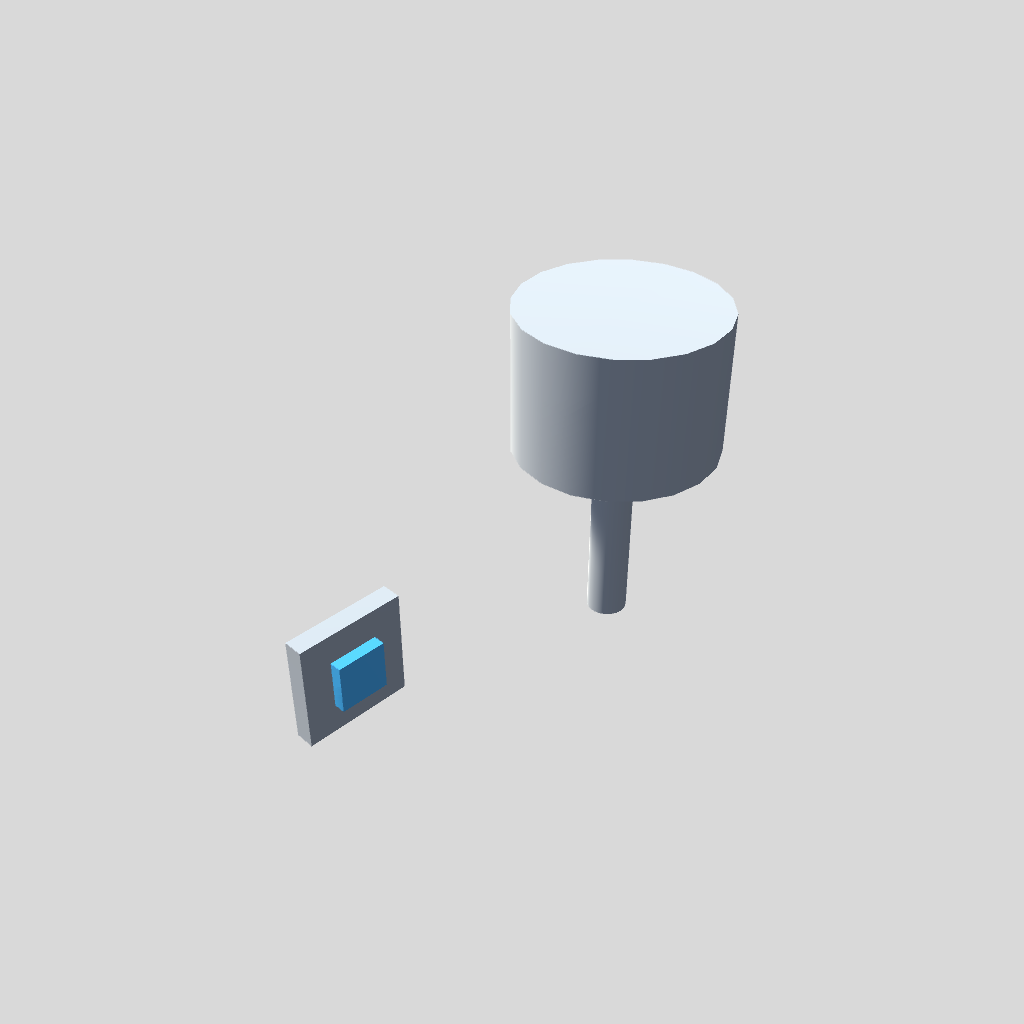
\includegraphics[width=0.3\linewidth]{figures/asset-examples-iso/Lamp_iso_top_right}\hfill
  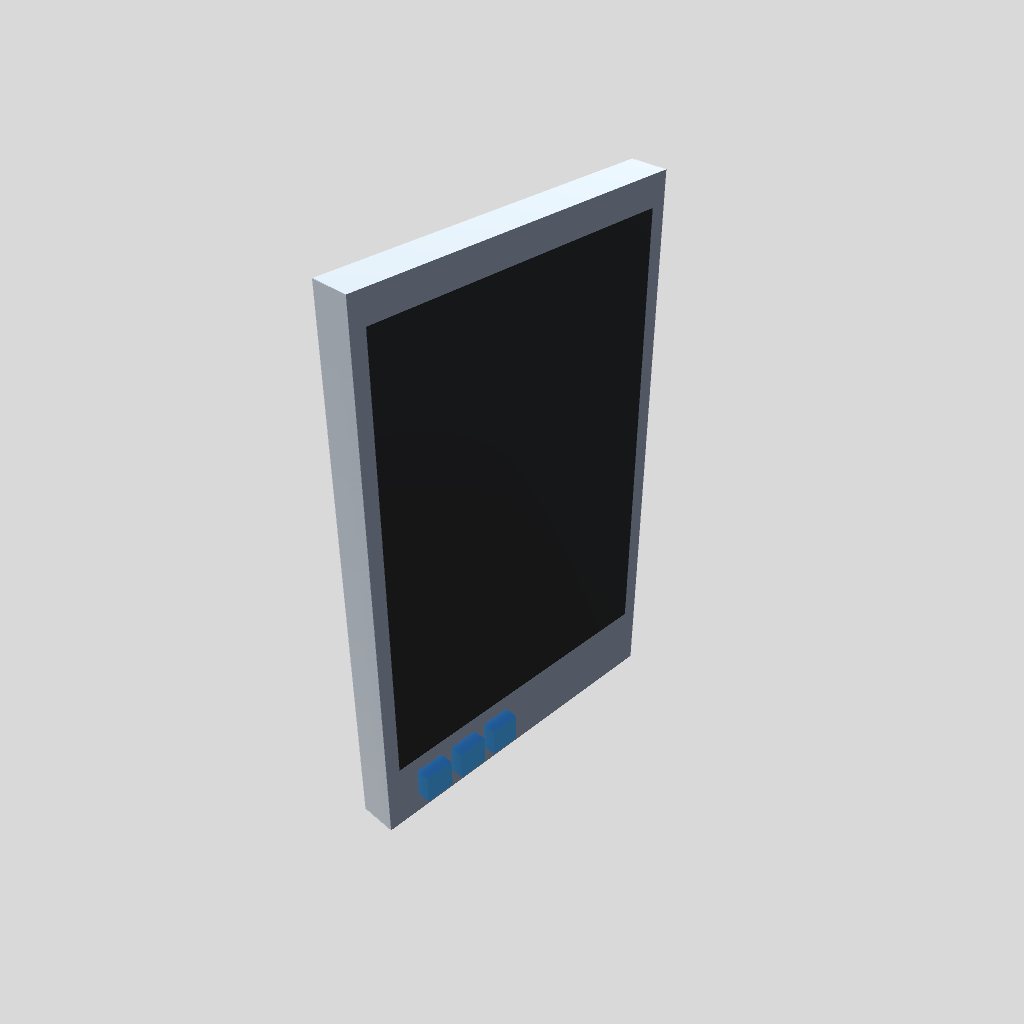
\includegraphics[width=0.3\linewidth]{figures/asset-examples-iso/Display_iso_top_right}\hfill
  \includegraphics[width=0.3\linewidth]{figures/asset-examples-iso/toaster3_iso_top_right}
  \caption{Die drei Testassets Lampe, Display und Toaster (von links nach rechts).}\label{fig:testasset_examples_iso}
\end{figure}

Die drei Assets unterscheiden sich hinsichtlich ihrer funktionalen sowie strukturellen Komplexität, wodurch der Workflow nicht nur an einem einfachen Erfolgsbeispiel, sondern anhand verschiedener Testfälle mit steigender Komplexität und Anforderungen gezeigt werden kann. Die Lampe bildet das einfachste Beispiel ab, da hier nur eine Interaktion sowie eine visuelle Reaktion erwartet werden. Einen mittleren Schwierigkeitsgrad stellt das Display dar, da hier verschiedene Bedienelemente und eine Screen-Fläche erkannt sowie in Beziehung zueinander gesetzt werden müssen. Abschließend bietet der Toaster das komplexeste Beispiel, da hier mehrere Teilobjekte, unterschiedliche visuelle Rückmeldungen, verschiedene Zustände sowie ein zeitbasierter Übergang miteinander funktionieren müssen.

Für die Bewertung der Pipeline sind verschiedene Kriterien relevant, anhand derer die Auswahl der Testassets erfolgte. Ein erstes Kriterium ist die Auswahl relevanter Teilobjekte. Je mehr Teilobjekte ein Asset besitzt, desto anspruchsvoller ist für den VSG, jene Bestandteile zu identifizieren, die tatsächlich relevant für die gewünschte Interaktion sind. Bei der Lampe betrifft das den Knopf sowie den Lampenschirm bzw. die Lichtquelle. Beim Display hingegen müssen bereits mehrere Bedienelemente sowie eine Screen-Fläche erkannt und unterschieden werden. Das Toaster-Beispiel enthält zusätzlich einen Hebel, eine Stopp-Taste sowie Heizelemente zur Visualisierung.

Ein zweites Kriterium beschreibt die Anzahl und Art der erwarteten Rollen. Nicht nur muss die Pipeline relevante Objektbestandteile erkennen, sondern diese später auch passenden funktionalen Vivian-Rollen zuordnen. Während die Lampe mit zwei Arten von Interaktions- sowie Visualisierungselementen (\textit{Button} und \textit{Light}) auskommt, benötigt das Display neben mehreren Eingabeelementen (\textit{Buttons}) auch ein Screen-Element, um Inhalte tatsächlich anzuzeigen. Beim Toaster müssen unterschiedliche Rollen erkannt werden, wie Hebel und Stopp-Taste als Bedienelemente (\textit{Slider} und \textit{Button}) sowie visuelle Elemente wie LED und Heizelemente als \textit{Lights}.

Auch die Komplexität der Interaktionslogik stellt ein Auswahlkriterium dar. Weniger komplexe Prototypen kommen mit weniger komplexer Logik aus. Beim Lampen-Beispiel schaltet ein Knopfdruck das Licht an oder aus. Komplexere Prototypen wie das Display benötigen wiederum bereits mehrere voneinander unterscheidbare Aktionen. Ein Knopf schaltet das Display an oder aus und weitere Knöpfe ermöglichen ein Wechseln zwischen verschiedenen Seiten. Der Toaster enthält zudem eine zeitbasierte Komponente, welche es ermöglicht, einen Toastvorgang wahlweise per Tastendruck oder nach einer fest definierten Zeit zu beenden. Dieser Fall umfasst nach direkten Interaktionen somit auch eine automatische Zustandsänderung nach Ablauf einer definierten Zeit.
Außerdem wurden unterschiedliche visuelle Rückmeldungen berücksichtigt. Für die Evaluation ist dies wichtig, da ein Prototyp intern korrekt umgesetzte Zustände und Zustandsübergänge nachvollziehbar für Nutzer*innen veranschaulichen soll. Die Lampe verwendet dafür das Leuchten des Lampenschirms. Das Display-Beispiel nutzt die Darstellung der Screen-Inhalte und der Toaster simuliert das Glühen der Heizelemente sowie das Leuchten einer LED während des Toastvorgangs.

\begin{table}[htbp]
  \centering
  \begin{tabularx}{\linewidth}{ll>{\raggedright\arraybackslash}X}
    \toprule
    Asset   & Komplexität & Erwartete Hauptfunktion                                                                                                                                                 \\
    \midrule
    Lampe   & leicht      & Der Lampenschirm soll als Lichtquelle leuchten. Ein Knopf soll die Lampe an- \bzw ausschalten.                                                                          \\
    Display & mittel      & Das Display soll ein- und ausgeschaltet werden können, Screen-Inhalte anzeigen sowie zwischen Seiten wechseln können.                                                   \\
    Toaster & schwer      & Der Toastvorgang soll durch den Hebel gestartet, mittels LED und Heizelementen visualisiert sowie nach zehn Sekunden oder durch Drücken der Stopp-Taste beendet werden. \\
    \bottomrule
  \end{tabularx}
  \caption{Übersicht der ausgewählten Testassets.}\label{tab:übersicht_testassets}
\end{table}

Die Assets wurden demnach so gewählt, dass sie eine aufsteigende Schwierigkeit abbilden. Sie reichen von einer einfachen Interaktion mit direkter visueller Rückmeldung über einen Prototypen mit mehreren Bedienelementen hin zu einem Objekt mit mehreren Funktionen, Zuständen und Übergängen. In der nachfolgenden Tabelle sind die ausgewählten Assets, ihre Komplexität sowie die jeweils erwartete Hauptfunktion zusammengefasst.




% \begin{table}[htbp]
%   \centering
%   \begin{tabularx}{\linewidth}{l>{\raggedright\arraybackslash}X>{\raggedright\arraybackslash}X>{\raggedright\arraybackslash}X}
%     \toprule
%     Aspekt
%      & Lampe
%      & Display
%      & Toaster                                                                                     \\
%     \midrule
%     Erwartete Teilobjekte
%      & Knopf, Lampenschirm
%      & Bedienknöpfe, Screen-Fläche
%      & Hebel, Stopp-Taste, Heizelemente, LED                                                       \\
%     \addlinespace
%     Erwatete Rollen
%      & \textit{Button}, \textit{Light}
%      & \textit{Buttons}, \textit{Screen}
%      & \textit{Slider} (Hebel), \textit{Button} (Stopp-Taste), \textit{Lights} (LED, Heizelemente) \\
%     \addlinespace
%     Erwartete Zustände
%      & an, aus
%      & aus, Seite~1, Seite~2
%      & idle, toasting                                                                              \\
%     \addlinespace
%     Erwartete Übergänge
%      & Knopfdruck schaltet zwischen an und aus um
%      & Ein-/Aus-Knopf wechselt Zustand, weitere Knöpfe wechseln zwischen den Seiten
%      & Hebel startet Toastvorgang; Stopp-Taste oder Ablauf von zehn Sekunden beendet ihn           \\
%     \addlinespace
%     Erwartete visuelle Reaktionen
%      & Lampenschirm leuchtet im Zustand \glqq an\grqq
%      & Screen zeigt im jeweiligen Zustand den passenden Inhalt
%      & LED leuchtet während des Toastvorgangs, Heizelemente glühen                                 \\
%     \bottomrule
%   \end{tabularx}
%   \caption{Übersicht der Referenzszenarien.}\label{tab:übersicht_referenzszenarien}
% \end{table}

% punkte 4-8

% 4: Lampe beschreiben
% 5: Display beschreiben
% 6: Toaster beschreiben

% evtl. 6.3 „Bewertungsmaßstäbe“ schreiben und mit 5/6/7 fortfahren
\section{Exemplarischer Workflow-Durchlauf}

Zunächst wird ein exemplarischer Einzeldurchlauf beschrieben, um die Funktionsweise des VSG nicht nur abstrakt, sondern anhand eines vollständigen Generierungsprozesses zu zeigen. Ziel ist die Nachvollziehbarkeit eines Durchlaufs von Eingabe bis validierter Spezifikation. Dafür wurde das Display-Asset ausgewählt, da es einen mittleren Schwierigkeitsgrad darstellt, mehrere Bedienelemente (\textit{Buttons}), eine Screen-Fläche als Visualisierungsobjekt und mehrere Zustände besitzt, aber noch übersichtlicher als das Toaster-Beispiel ist. Die Hierarchie des Display-Assets ist in Abbildung~\ref{fig:display_asset_treeview} abgebildet und zeigt die verschiedenen Bedienelemente sowie die Screen-Fläche. Die natürlichsprachliche Eingabe in der Vorverarbeitung sowie die Prüfung des Interaktionsplans durch Benutzende zeigt den Co-Creation-Workflow. Weiterhin wird gezeigt, dass Teilobjekte und Elementrollen von der Pipeline erkannt werden. Indem Zustände, Übergänge sowie sichtbare Screen-Wechsel vom VSG geplant und schließlich umgesetzt werden, wird gezeigt, dass Interaktionslogiken aus der natürlichsprachlichen Interaktionsbeschreibung und bestehenden 3D-Geometrien extrahiert und in eine maschinenlesbare Repräsentation überführt werden können. Der hier betrachtete Fall stellt eine positive Referenz dar, da der Durchlauf im ersten Versuch zu einer validierten Vivian-Spezifikation gelangte. In diesem Unterkapitel wird zunächst die grundlegende Machbarkeit des Workflows gezeigt. Es wird daraus jedoch noch keine allgemeine Aussage über die Robustheit oder Wiederholbarkeit abgeleitet, dazu werden anschließend mehrere Durchläufe betrachtet.

\begin{figure}[htbp]
  \centering
  \begin{forest}
    for tree={
        font=\ttfamily,
        grow'=0,
        folder,
        fit=band,
        s sep=2pt,
      }
      [Display
          [DisplayHousing
              [DisplayPlane
                  [DisplayContent]
              ]
              [Frame]
          ]
          [Controls
              [ButtonBack]
              [ButtonPower]
              [ButtonForward]
          ]
      ]
  \end{forest}
  \caption{Hierarchie des Display-Assets in der Unity-Szene}\label{fig:display_asset_treeview}
\end{figure}


Die KI-gestützte Pipeline erhielt die vorverarbeitete Szene, bestehend aus JSON- und Bilddateien, drei Bilddateien, um diese auf dem Bildschirm anzuzeigen, sowie eine natürlichsprachliche Beschreibung des gewünschten Verhaltens. Darin wurde das Asset als Display mit drei Knöpfen zur Steuerung und einem Bildschirm beschreiben. Die Knöpfe sollten dazu dienen, das Display ein- und auszuschalten sowie zum vorherigen beziehungsweise zum nächsten Bild zu wechseln. Zusätzlich wurde festgelegt, dass die Navigation durch die Bilddateien endlos stattfinden soll, sodass Bild drei beispielsweise über eine Vorwärtsnavigation wieder zu Bild eins wechselt. Aus dieser Beschreibung ergab sich vorab ein Referenzszenario mit vier Teilobjekten. Diese sowie deren erwartete Kategorie und Vivian-Rollen sind der folgenden Tabelle zu entnehmen.

\begin{table}[htbp]
  \centering
  \begin{tabularx}{\linewidth}{l>{\raggedright\arraybackslash}X>{\raggedright\arraybackslash}X}
    \toprule
    Teilobjekt     & Kategorie      & Vivian-Rolle \\
    \midrule
    ButtonBack     & Interaktion    & Button       \\
    ButtonPower    & Interaktion    & ToggleButton \\
    ButtonForward  & Interaktion    & Button       \\
    DispalyContent & Visualisierung & Screen       \\
    \bottomrule
  \end{tabularx}
  \caption{Erwartete Teilobjekte, Kategorien und Vivian-Rollen des Display-Assets.}\label{tab:display_teilobjekte}
\end{table}

Weiterhin wurden vier erwartete Zustände definiert: ein Zustand, in dem der Bildschirm ausgeschaltet ist und kein Bild angezeigt wird sowie ein Zustand je anzuzeigendem Bild. Aus diesen Zuständen ergaben sich weiterhin zehn erwartete Übergänge. Der Power-Button sollte aus dem ausgeschalteten Zustand in einen den ersten Bildzustand wechseln sowie aus jedem Bildzustand zurück in den ausgeschalteten Zustand. Der Button zur Vorwärtsnavigation sollte von Bild eins zu Bild zwei, von Bild zwei zu Bild drei, und schließlich wieder von Bild 3 zu Bild eins wechseln, um ein zyklisches Wechseln zwischen den Bildern zu ermöglichen. Der Button zur Rückwärtsnavigation sollte dieselbe Bildmenge in umgekehrter Richtung durchlaufen. Die erwarteten Zustände und Übergänge sind außerdem in der folgenden Tabelle zusammengefasst.

\begin{table}[htbp]
  \centering
  \begin{tabularx}{\linewidth}{l>{\raggedright\arraybackslash}X}
    \toprule
    Name       & Beschreibung                                             \\
    \midrule
    powerOff   & Bildschirm ausgeschaltet, kein Bildinhalt                \\
    imageOne   & Bildschirm angeschaltet, Anzeige des ersten Bildinhalts  \\
    imageTwo   & Bildschirm angeschaltet, Anzeige des zweiten Bildinhalts \\
    imageThree & Bildschirm angeschaltet, Anzeige des dritten Bildinhalts \\
    \bottomrule
  \end{tabularx}
  \caption{Erwartete Zustände des Display-Assets.}\label{tab:display_zustaende}
\end{table}

\begin{table}[htbp]
  \centering
  \begin{tabular}{lll}
    \toprule
    Ausgangszustand & Zielzustand & Auslöser      \\
    \midrule
    powerOff        & imageOne    & ButtonPower   \\
    imageOne        & powerOff    & ButtonPower   \\
    imageTwo        & powerOff    & ButtonPower   \\
    imageThree      & powerOff    & ButtonPower   \\
    imageOne        & imageTwo    & ButtonForward \\
    imageTwo        & imageThree  & ButtonForward \\
    imageThree      & imageOne    & ButtonForward \\
    imageOne        & imageThree  & ButtonBack    \\
    imageTwo        & imageOne    & ButtonBack    \\
    imageThree      & imageTwo    & ButtonBack    \\
    \bottomrule
  \end{tabular}
  \caption{Erwartete Übergänge des Display-Assets.}\label{tab:display_uebergaenge}
\end{table}





\chapter{Ausblick und Fazit}\label{ch:ausblick_fazit}
\include{content/8_fazit}

% remove if not needed
\appendix
\chapter{Agenten-Instruktionen}\label{ch:anhang_agenten_instruktionen}

\section{Scene Analysis Agent}\label{sec:anhang_scene_analysis_instructions}

Die folgende Instruktion wird dem \textit{scene\_analysis\_agent} als Systemprompt übergeben.
Sie definiert Eingaben, Ausgabeformat sowie die Heuristiken zur Inferenz der Interaktionsachse.

\lstinputlisting[
    basicstyle=\ttfamily\footnotesize,
    breaklines=true,
    breakatwhitespace=true,
    columns=fullflexible,
    frame=single,
    numbers=none,
    showstringspaces=false,
    keepspaces=true,
    inputencoding=utf8,
    extendedchars=true,
    literate={≈}{{$\approx$}}1 {→}{{$\rightarrow$}}1 {—}{{---}}1 {–}{{--}}1 {„}{{\quotedblbase}}1 {“}{{\textquotedblleft}}1 {”}{{\textquotedblright}}1 {‚}{{\quotesinglbase}}1 {‘}{{\textquoteleft}}1 {’}{{\textquoteright}}1 {ä}{{\"a}}1 {ö}{{\"o}}1 {ü}{{\"u}}1 {Ä}{{\"A}}1 {Ö}{{\"O}}1 {Ü}{{\"U}}1 {ß}{{\ss}}1
]{appendix/scene-analysis-instr.txt}


\backmatter
\listoffigures
\cleardoublepage

\listoftables
\cleardoublepage

\renewcommand{\lstlistlistingname}{Listingverzeichnis}
\lstlistoflistings
\cleardoublepage

\printbibliography

% \printnoidxglossaries
\printglossary

\end{document}
